\documentclass[a4paper,12pt,twoside]{memoir}
\let\footruleskip\undefined	% see http://tex.stackexchange.com/questions/37868/fancyhdr-and-memoir
\usepackage{fancyhdr}	% For headers and footers
\usepackage{listings}	% Required for insertion of code
\usepackage{courier}	% Required for the courier font
\usepackage[usenames,dvipsnames]{color} % Required for custom colors
\usepackage[table]{xcolor}
\usepackage[pdftex]{graphicx}
\usepackage{hyperref}
\usepackage{fullpage}	% See http://en.wikibooks.org/wiki/LaTeX/Page_Layout#Manual_Page_Formatting for layout
\usepackage{enumitem}
%\usepackage[parfill]{parskip}	% Don't indent the first line of paragraphs
\linespread{1.0} % Line spacing
\usepackage{mdframed}
%\usepackage{parskip}
\usepackage{etoolbox}
\usepackage[nobottomtitles]{titlesec}
\usepackage[section]{placeins}
\setlength{\parindent}{0pt}
\usepackage{ifthen}
\usepackage{array}
% packages for Creative Commons Licences
\usepackage{xmpincl}
\includexmp{licences/CC_Attribution_3.0_Unported}	% includes XML metadata into the PDF
%\usepackage{scrextend}
\usepackage{microtype}
\usepackage{accsupp}
\usepackage{textcomp}
\usepackage{float}
\usepackage{lmodern}        % to ensure most charaters in listings and texttt are copy-paste safe and print nicely
\usepackage{comment}
\newtoggle{trainermanual}   % defaults to false


\settoggle{trainermanual}{false}  % Uncomment to generate the trainer's manual

\raggedbottom               % put all vertical white space at the bottom of the page 

\newlength{\defparskip}
\setlength{\defparskip}{0.5cm}
\specialcomment{answer}{\begingroup\color{red}}{\endgroup}

\newlength{\descriptionlabelspace}
\setlength{\descriptionlabelspace}{5.5cm}

% config display of hyperlinks
\hypersetup{
    colorlinks=true,		    % false: boxed links; true: colored links
    linkcolor=red,          % color of internal links
    citecolor=green,        % color of links to bibliography
    filecolor=magenta,      % color of file links
    urlcolor=blue           % color of external links
}

\definecolor{darkgreen}{rgb}{0,0.9,0}
\newcommand{\noncopytext}[1]{%
    \BeginAccSupp{method=escape,ActualText={}}%
    #1%
    \EndAccSupp{}%
}
\lstset{ %
%    language=sh,                    % the language of the code
    columns=fullflexible,
    upquote=true,
    aboveskip=5pt,
    belowskip=10pt,
    basicstyle=\small\ttfamily,      % the size of the fonts that are used for the code
    numbers=left,                    % where to put the line-numbers
    numberstyle=\tiny\color{black!85}\noncopytext,  % the style that is used for the line-numbers
    stepnumber=1,                    % the step between two line-numbers. If it's 1, each line 
%                                    % will be numbered
    numbersep=13pt,                  % how far the line-numbers are from the code. Add framesep value to this
    backgroundcolor=\color{black!5}, % choose the background color. You must add \usepackage{color}
    showspaces=false,                % show spaces adding particular underscores
    showstringspaces=false,          % underline spaces within strings
    showtabs=false,                  % show tabs within strings adding particular underscores
    xleftmargin=20pt,
    xrightmargin=10pt,
    framesep=5pt,
    framerule=3pt,
    frame=leftline,                  % adds a frame around the code
    rulecolor=\color{darkgreen},     % if not set, the frame-color may be changed on line-breaks within not-black text (e.g. commens (green here))
    tabsize=2,                       % sets default tabsize to 2 spaces
    breaklines=true,                 % sets automatic line breaking
    breakatwhitespace=true,          % sets if automatic breaks should only happen at whitespace
    breakindent=20pt,
    breakautoindent=true,
    prebreak=\small\symbol{'134},
    literate=%{*}{{\textasteriskcentered}}{1}
             {~}{{\texttildelow}}{1} % reformat the high tilde to a normal tile which looks good for printing and is copy-and-pastable
             %{-}{{\textminus}}{1},
}

% configure an R listings
%\lstloadlanguages{R}
% \lstdefinelanguage{Renhanced}[]{R}{%
%   morekeywords={acf,ar,arima,arima.sim,colMeans,colSums,is.na,is.null,%
%     mapply,ms,na.rm,nlmin,replicate,row.names,rowMeans,rowSums,seasonal,%
%     sys.time,system.time,ts.plot,which.max,which.min},
%   deletekeywords={c},
%   alsoletter={.\%},%
%   alsoother={:_\$}}
% \lstset{language=Renhanced,extendedchars=true,
%   basicstyle=\small\ttfamily,
%   commentstyle=\textsl,
%   keywordstyle=\mdseries,
%   showstringspaces=false,
%   index=[1][keywords], 
%   indexstyle=\indexfonction}

% disables chapter, section and subsection numbering
% and number figures and tables consecutively throughout the document
\setcounter{secnumdepth}{-1}
\counterwithout{figure}{chapter}
\counterwithout{table}{chapter}


% This allows stuff on the same line to be vertically centered with respect of each other
\def\vcent#1{\mathsurround0pt$\vcenter{\hbox{#1}}$}
\def\vtp#1{\mathsurround0pt$\vtop{\hbox{#1}}$}

% config ...
\setlength{\topskip}{0.75cm}
\definecolor{warningshade}{rgb}{1,0.85,0.85}
\definecolor{questionshade}{rgb}{1,0.95,0.85}
\definecolor{bonusshade}{rgb}{0.92,1,0.92}
\definecolor{advancedshade}{rgb}{0.92,0.92,1}

% defaine a default style for the mdframed-based environments
% TODO Figure out how to apply the default style as the basis for other styles
\global\mdfdefinestyle{default}{
  leftmargin=0pt,
  skipabove=5pt,
  rightmargin=0pt,
  skipbelow=10pt,
  %splittopskip=0pt,
  %splitbottomskip=0pt,
  innermargin=0pt,
  outermargin=0pt,
  innerleftmargin=0pt,
  innerrightmargin=0pt,
  innertopmargin=0pt,
  innerbottommargin=0pt,
  leftline=false,
  topline=false,
  rightline=false,
  bottomline=false,
  linecolor=black,
  linewidth=1pt,
  roundcorner=5pt,
}

\global\mdfdefinestyle{warningbox}{
  leftmargin=0pt,
  skipabove=5pt,
  rightmargin=0pt,
  skipbelow=10pt,
  %splittopskip=0pt,
  %splitbottomskip=0pt,
  innermargin=0pt,
  outermargin=0pt,
  innerleftmargin=0pt,
  innerrightmargin=0pt,
  innertopmargin=0pt,
  innerbottommargin=0pt,
  leftline=false,
  topline=false,
  rightline=false,
  bottomline=false,
  linecolor=black,
  linewidth=1pt,
  roundcorner=5pt,
  backgroundcolor=warningshade,
  leftline=true,
  topline=true,
  rightline=true,
  bottomline=true,
  innerleftmargin=10pt,
  innerrightmargin=10pt,
  innertopmargin=10pt,
  innerbottommargin=10pt,
  nobreak=true,
}
\global\mdfdefinestyle{questionsbox}{
  leftmargin=0pt,
  skipabove=5pt,
  rightmargin=0pt,
  skipbelow=10pt,
  %splittopskip=0pt,
  %splitbottomskip=0pt,
  innermargin=0pt,
  outermargin=0pt,
  innerleftmargin=0pt,
  innerrightmargin=0pt,
  innertopmargin=0pt,
  innerbottommargin=0pt,
  leftline=false,
  topline=false,
  rightline=false,
  bottomline=false,
  linecolor=black,
  linewidth=1pt,
  roundcorner=5pt,
  backgroundcolor=questionshade,
  leftline=true,
  topline=true,
  rightline=true,
  bottomline=true,
  innerleftmargin=10pt,
  innerrightmargin=10pt,
  innertopmargin=10pt,
  innerbottommargin=10pt,
  skipabove=15pt,
  skipbelow=20pt,
  nobreak=true,
}
\global\mdfdefinestyle{bonusbox}{
  leftmargin=0pt,
  skipabove=5pt,
  rightmargin=0pt,
  skipbelow=10pt,
  %splittopskip=0pt,
  %splitbottomskip=0pt,
  innermargin=0pt,
  outermargin=0pt,
  innerleftmargin=0pt,
  innerrightmargin=0pt,
  innertopmargin=0pt,
  innerbottommargin=0pt,
  leftline=false,
  topline=false,
  rightline=false,
  bottomline=false,
  linecolor=black,
  linewidth=1pt,
  roundcorner=5pt,
%  backgroundcolor=bonusshade,
  leftline=true,
  topline=true,
  rightline=true,
  bottomline=true,
  innerleftmargin=10pt,
  innerrightmargin=10pt,
  innertopmargin=10pt,
  innerbottommargin=10pt,
  skipabove=15pt,
  skipbelow=20pt,
  nobreak=false,                % these could span multiple pages, so we should let them break across pages
}
\global\mdfdefinestyle{advancedbox}{
  leftmargin=0pt,
  skipabove=5pt,
  rightmargin=0pt,
  skipbelow=10pt,
  %splittopskip=0pt,
  %splitbottomskip=0pt,
  innermargin=0pt,
  outermargin=0pt,
  innerleftmargin=0pt,
  innerrightmargin=0pt,
  innertopmargin=0pt,
  innerbottommargin=0pt,
  leftline=false,
  topline=false,
  rightline=false,
  bottomline=false,
  linecolor=black,
  linewidth=1pt,
  roundcorner=5pt,
%  backgroundcolor=advancedshade,
  leftline=true,
  topline=true,
  rightline=true,
  bottomline=true,
  innerleftmargin=10pt,
  innerrightmargin=10pt,
  innertopmargin=10pt,
  innerbottommargin=10pt,
  skipabove=15pt,
  skipbelow=20pt,
  nobreak=false,                % these could span multiple pages, so we should let them break across pages
}

\newlength{\iconspacinglength}
\setlength{\iconspacinglength}{0.5cm}
\newcommand{\iconspacing}{\iconspacinglength}
\newlength{\questionspacing}
\setlength{\questionspacing}{2cm}


\newenvironment{steps}{%
\begin{mdframed}[style=default]%
%\addtolength{\iconspacinglength}{\mdflength{leftmargin}}%
%\addtolength{\iconspacinglength}{\mdflength{innerleftmargin}}%
\makebox[0pt][r]{\smash{\raisebox{-.6\height}{%

\includegraphics[height=1cm]{./graphics/steps.png}%
\hspace{\iconspacinglength}%
}}}\ignorespaces%
}%
{%
\end{mdframed}%
}

\newenvironment{bonus}{%
\begin{mdframed}[style=bonusbox]%
\addtolength{\iconspacinglength}{\mdflength{leftmargin}}%
\addtolength{\iconspacinglength}{\mdflength{innerleftmargin}}%
%\newpage%
\makebox[0pt][r]{\smash{\raisebox{-.6\height}{%

\includegraphics[height=1cm]{./graphics/bonus1.png}%
\hspace{\iconspacinglength}%
}%
}%
}\ignorespaces%\vspace{-3em}\vspace{-\parskip}%
}%
{%
\end{mdframed}%
}
  
\newenvironment{advanced}{%
\begin{mdframed}[style=advancedbox]%
\addtolength{\iconspacinglength}{\mdflength{leftmargin}}%
\addtolength{\iconspacinglength}{\mdflength{innerleftmargin}}%
%\newpage%
\makebox[0pt][r]{\smash{\raisebox{-.6\height}{%

\includegraphics[height=1cm]{./graphics/bonus2.png}%
\hspace{\iconspacinglength}%
}%
}%
}\ignorespaces%\vspace{-3em}%
}%
{%
\end{mdframed}%
}

\newenvironment{information}{%
\begin{mdframed}[style=default]%
%\addtolength{\iconspacinglength}{\mdflength{leftmargin}}%
%\addtolength{\iconspacinglength}{\mdflength{innerleftmargin}}%
\makebox[0pt][r]{\smash{\raisebox{-.6\height}{%

\includegraphics[height=1cm]{./graphics/info.png}%
\hspace{\iconspacinglength}%
}}}\ignorespaces%
}%
{%
\end{mdframed}%
}

\newenvironment{note}{%
\begin{mdframed}[style=default]%
%\addtolength{\iconspacinglength}{\mdflength{leftmargin}}%
%\addtolength{\iconspacinglength}{\mdflength{innerleftmargin}}%
\makebox[0pt][r]{\smash{\raisebox{-.6\height}{%

\includegraphics[height=1cm]{./graphics/notes.png}%
\hspace{\iconspacinglength}%
}}}\ignorespaces%
}%
{%
\end{mdframed}%
}

\newenvironment{warning}{%
\begin{mdframed}[style=warningbox]%
\addtolength{\iconspacinglength}{\mdflength{leftmargin}}%
\addtolength{\iconspacinglength}{\mdflength{innerleftmargin}}%
\makebox[0pt][r]{\smash{\raisebox{-.25\height}{%

\includegraphics[height=1cm]{./graphics/warning.png}%
\hspace{\iconspacinglength}%
}}}\ignorespaces%
}%
{%
\end{mdframed}%
}

\newenvironment{questions}{%
\begin{mdframed}[style=questionsbox]%
\nottoggle{trainermanual}{\setlength{\parskip}{\questionspacing}}{}%
\addtolength{\iconspacinglength}{\mdflength{leftmargin}}%
\addtolength{\iconspacinglength}{\mdflength{innerleftmargin}}%
\makebox[0pt][r]{\smash{\raisebox{-.25\height}{%

\includegraphics[height=1cm]{./graphics/questions.png}%
\hspace{\iconspacinglength}%
}}}\ignorespaces%
}%
{%
\nottoggle{trainermanual}{\vspace{\questionspacing}}{}%
\end{mdframed}%
}

\definecolor{trainerfrontpageshade}{rgb}{1,0.9,0.9}
\newcommand{\trainermanualtext}{\huge\textbf{\textcolor{red}{TRAINER'S MANUAL}}}


\newcommand{\workshoptitlepage}{
\thispagestyle{plain}
\iftoggle{trainermanual}{
\pagecolor{trainerfrontpageshade}
}{}
\noindent

\begin{center}
\rule{\textwidth}{1pt}

\vspace*{\fill}
{\Huge\workshopTitle}
\vspace{2cm}

\workshopAuthor

\vfill

\rule{\textwidth}{1pt}
\begin{minipage}{0.45\textwidth}
\begin{flushleft}
\workshopVenue
\end{flushleft}
\end{minipage}
\begin{minipage}{0.45\textwidth}
\begin{flushright}
\workshopDate
\end{flushright}
\end{minipage}
\rule{\textwidth}{1pt}
\end{center}
\clearpage
\iftoggle{trainermanual}{
\pagecolor{white}%
}{}
}

%TODO Revise this chapter styling code, there appears to be a couple of things wrong with it.
\makechapterstyle{workshop}{%
  \chapterstyle{default}
  \renewcommand*{\chapnumfont}{\normalfont\HUGE\sffamily}
  \renewcommand*{\chaptitlefont}{\normalfont\huge\sffamily}
  \settowidth{\chapindent}{\chapnumfont 111}
  \renewcommand*{\chapterheadstart}{\begingroup
    %\vspace*{\beforechapskip}%
    \begin{adjustwidth}{}{-\chapindent}%
    \hrulefill
    \smash{\rule{0.4pt}{15mm}}
    \end{adjustwidth}\endgroup}
  \renewcommand*{\printchaptername}{}
  \renewcommand*{\chapternamenum}{}
  \renewcommand*{\printchapternum}{%
    \begin{adjustwidth}{}{-\chapindent}
    \hfill
    \raisebox{10mm}[0pt][0pt]{\chapnumfont \thechapter}%
                              \hspace*{1em}
    \end{adjustwidth}\vspace*{-3.0\onelineskip}}
  \renewcommand*{\printchaptertitle}[1]{%
    \vskip\onelineskip
    \raggedleft {\chaptitlefont ##1}\par\nobreak}
  
}
\makechapterstyle{module}{%
  \chapterstyle{workshop}
  \renewcommand*{\printchaptertitle}[1]{%
    \vskip\onelineskip
    \raggedleft {\chaptitlefont Module: ##1}\par\nobreak
    \vspace{\vfill}
    Primary Author(s):\par
    \moduleAuthors\par
    \vspace{1cm}
    Contributor(s):\par
    \moduleContributions}\par
}
\aliaspagestyle{chapter}{empty}
\newcommand{\mailto}[1]{
\href{mailto:#1}{\nolinkurl{#1}}
}

\newcommand{\moduleTitle}{}
\newcommand{\moduleAuthors}{}
\newcommand{\moduleContributions}{}

%\newcolumntype{V}{>{\centering\arraybackslash} m{3cm} }

%
% Some User Defined Stuff
%
\newcommand{\workshopTitle}{Introduction to Next Generation Sequencing Hands-on Workshop}
\newcommand{\workshopVenue}{Brisbane and Adelaide, Australia}
\newcommand{\workshopDate}{Nov. 2012}
\newcommand{\workshopAuthor}{
Bioplatforms Australia (BPA)\\
The Commonwealth Scientific and Industrial Research Organisation (CSIRO)\\
%The European BioinformaticsInstitute (EBI)\\
}
%
% End User Defined Stuff
%

% set default headers footers
\pagestyle{fancy}
\setlength{\headheight}{15pt}
\fancyhead[LE,RO]{\slshape \nouppercase{\leftmark}}
\fancyhead[LO,RE]{\slshape \nouppercase{\rightmark}}
\fancyfoot[LE,RO]{\thepage}
\fancyfoot[C]{}
\addtolength{\headsep}{\baselineskip} 
\iftoggle{trainermanual}{
\fancyfoot[C]{\trainermanualtext}
}{}

% define the plain page style for both trainee and trainer's manual
\fancypagestyle{plain}{%
\fancyhf{} % clear all header and footer fields
\renewcommand{\headrulewidth}{0pt}
}
\iftoggle{trainermanual}{
\fancypagestyle{plain}{%
\fancyhf{}
\fancyhead[C]{\trainermanualtext}
\fancyfoot[C]{\trainermanualtext}
\renewcommand{\headrulewidth}{0pt}
}{}
}


\title{\workshopTitle}
\date{\workshopDate}
\author{\workshopAuthor}


\nottoggle{trainermanual}{
\excludecomment{answer}
}{}

%\includeonly{workshop_preamble.tex,rna-seq.tex}

\chapterstyle{workshop}

\begin{document}

%
% Workshop Title Page
%
\workshoptitlepage

%
% CC-BY
%
\chapter{Licensing}

This work is licensed under a Creative Commons Attribution 3.0 Unported License and
the below text is a summary of the main terms of the full Legal Code (the full licence) available at
\url{http://creativecommons.org/licenses/by/3.0/legalcode}.

\begin{description}[style=multiline,labelindent=0cm,align=left,leftmargin=1.5cm]
\item[You are free:] \hfill

to copy, distribute, display, and perform the work 

to make derivative works

to make commercial use of the work
  
\item[Under the following conditions:] \hfill

  \textbf{Attribution} - You must give the original author credit.
  
\item[With the understanding that:] \hfill

  \textbf{Waiver} - Any of the above conditions can be waived if you get permission from the
  copyright holder.
  
  \textbf{Public Domain} - Where the work or any of its elements is in the public domain
  under applicable law, that status is in no way affected by the license.
  
  \textbf{Other Rights} - In no way are any of the following rights affected by the license:
  
  \begin{itemize}
    \item Your fair dealing or fair use rights, or other applicable copyright exceptions and limitations;
  
    \item The author's moral rights;
  
    \item Rights other persons may have either in the work itself or in how the work is used, such
    as publicity or privacy rights.
  \end{itemize}
  
  \textbf{Notice} - For any reuse or distribution, you must make clear to others the
  licence terms of this work.
  
\end{description}

\vspace{\fill}

\begin{center}

\includegraphics[height=1cm]{./licences/cc_by.png}
\end{center}


\clearpage
\tableofcontents

\chapter{Workshop Information}

%
% Trainers Page
%
\section{The Trainers}

\newlength{\trainerIconWidth}
\setlength{\trainerIconWidth}{2.0cm}

\begin{table}[H]
  \centering
  \small
  \renewcommand{\arraystretch}{1}
  %\caption{A table arranging  images}
  \rowcolors{1}{gray!25}{white}
  \begin{tabular}{>{\centering\arraybackslash} m{1.1\trainerIconWidth} m{1\textwidth}}
    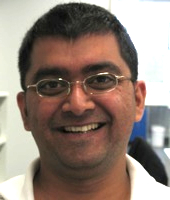
\includegraphics[width=\trainerIconWidth]{graphics/Deshpande.jpg} & 
      \textbf{Dr. Nandan Deshpande}\newline
      
      Postdoctoral Fellow\newline
      The University of New South Wales (UNSW), NSW\newline
      \mailto{n.deshpande@unsw.edu.au}\\
    
    
\includegraphics[width=\trainerIconWidth]{graphics/Duesing.jpg} & 
      \textbf{Dr. Konsta Duesing}\newline
      
      Research Team Leader - Statistics \& Bioinformatics\newline
      CSIRO Animal, Food and Health Science, NSW\newline
      \mailto{konsta.duesing@csiro.au}\\
    
    
\includegraphics[width=\trainerIconWidth]{graphics/Li.jpg} & 
      \textbf{Dr. Xi (Sean) Li}\newline
      
      Bioinformatics Analyst\newline
      Bioinformatics Core, CSIRO Mathematics, Informatics and Statistics, ACT\newline
      \mailto{sean.li@csiro.au}\\
    
    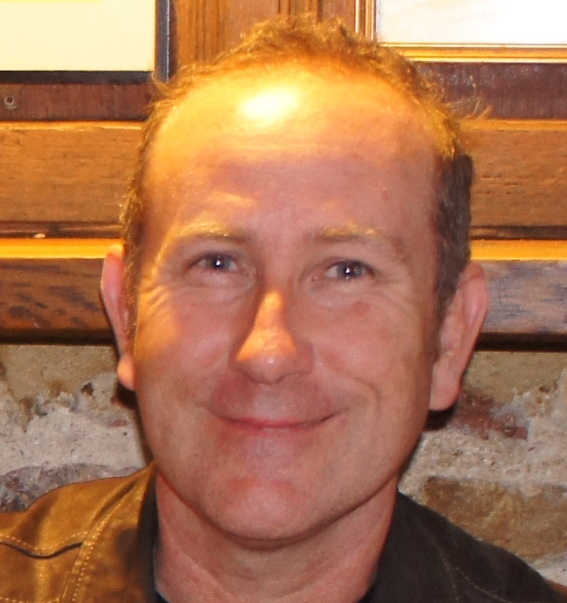
\includegraphics[width=\trainerIconWidth]{graphics/McWilliam.jpg} & 
      \textbf{Mr. Sean McWilliam}\newline
      
      Bioinformatics Analyst\newline
      CSIRO Animal, Food and Health Sciences, QLD\newline
      \mailto{sean.mcwilliam@csiro.au}\\
    
    
\includegraphics[width=\trainerIconWidth]{graphics/Moolhuijzen.jpg} & 
      \textbf{Dr. Paula Moolhuijzen}\newline
      
      Senior Bioinformatics Officer\newline
      Centre for Comparative Genomics, Murdoch University, WA\newline
      \mailto{pmoolhuijzen@ccg.murdoch.edu.au}\\
    
    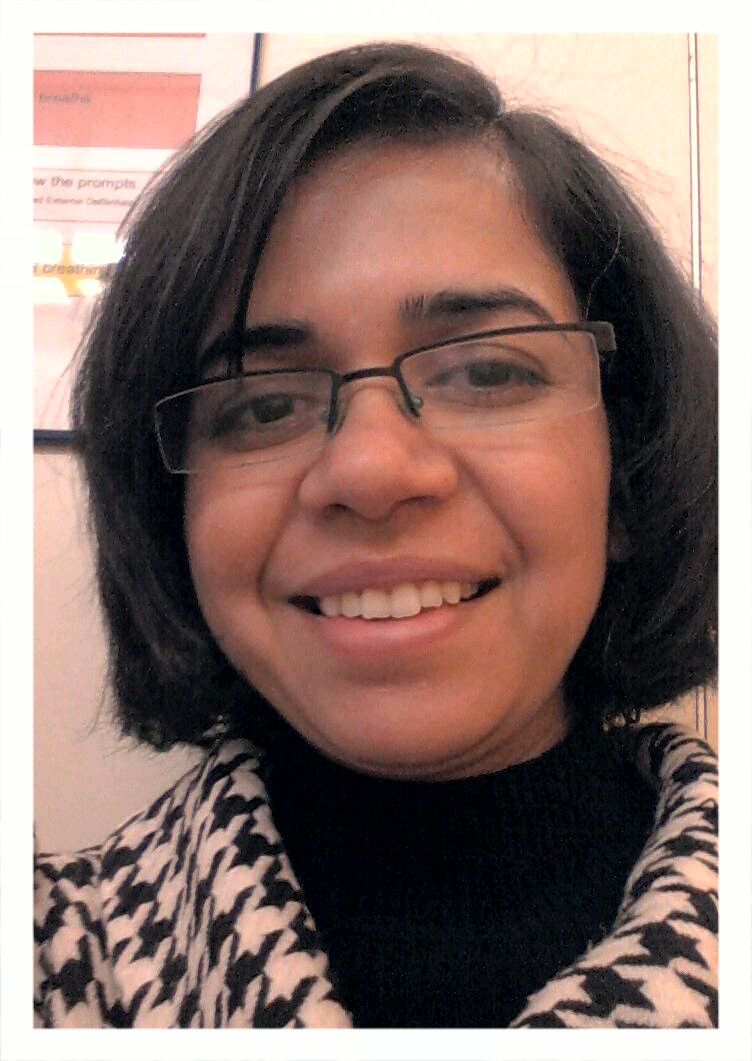
\includegraphics[width=\trainerIconWidth]{graphics/Tyagi.jpg} & 
      \textbf{Dr. Sonika Tyagi}\newline
      
      Senior Bioinformatics Officer\newline
      Australian Genome Research Facility Ltd, The Walter and Eliza Hall Institute, VIC\newline
      \mailto{sonika.tyagi@agrf.org.au}\\
    
    
\includegraphics[width=\trainerIconWidth]{graphics/watson-haigh.jpeg} & 
      \textbf{Dr. Nathan S. Watson-Haigh}\newline
      
      Research Fellow in Bioinformatics\newline
      The Australian Centre for Plant Functional Genomics (ACPFG), SA\newline
      \mailto{nathan.haigh@acpfg.com.au}\\
    
    \end{tabular}
  \caption{\label{tab:trainers}}
\end{table}


%
% Workshop Preamble
%
%
% Start: General Information describing the workshop and the structure of the handouts
%
\newpage

% \section{Do's and Don'ts of the Workshop}
% TODO Add do's and don'ts e.g. email, social media etc 

\section{Document Structure}
We have provided you with an electronic copy of the workshop's hands-on tutorial documents.
We have done this for two reasons: 1) you will have something to take away with you at the 
end of the workshop, and 2) you can save time (mis)typing commands on the command line by using
copy-and-paste.

\begin{warning}
While you could fly through the hands-on sessions doing
copy-and-paste you will learn more if you take the time, saved from not having to type all those
commands, to understand what each command is doing!
\end{warning}

The commands to enter at a terminal look something like this:
\begin{lstlisting}
tophat --solexa-quals -g 2 --library-type fr-unstranded -j annotation/Danio_rerio.Zv9.66.spliceSites -o tophat/ZV9_2cells genome/ZV9 data/2cells_1.fastq data/2cells_2.fastq
\end{lstlisting}  

The following icons are used in the margin, throughout the documentation to help you locate:

% TODO limit the use of some icons throughout as some are clearly overused and confuse the eye
\hspace*{.2cm}\vcent{
\includegraphics[height=1cm]{./graphics/info.png}} Important\\
\hspace*{.2cm}\vcent{
\includegraphics[height=1cm]{./graphics/notes.png}} For reference\\
\hspace*{.2cm}\vcent{
\includegraphics[height=1cm]{./graphics/steps.png}} Follow these steps\\
\hspace*{.2cm}\vcent{
\includegraphics[height=1cm]{./graphics/questions.png}} Questions to answer\\
\hspace*{.2cm}\vcent{
\includegraphics[height=1cm]{./graphics/warning.png}} Warning - STOP and read\\
\hspace*{.2cm}\vcent{
\includegraphics[height=1cm]{./graphics/bonus1.png}} Bonus exercise for fast learners\\
\hspace*{.2cm}\vcent{
\includegraphics[height=1cm]{./graphics/bonus2.png}} Advanced exercise for super-fast learners\\

\section{Resources Used}
We have provided you with an environment which contains all the tools and data
you need for the duration of this workshop. However, we also provide details
about the tools and data used by each module at the start of the respective
module documentation.


%
% Start of modules
% Switch chapter styling to module
%
\chapterstyle{module}

%
% QC Module
%
% Define the top matter
\renewcommand{\moduleTitle}{Data Quality}
\renewcommand{\moduleAuthors}{%
  Sonika Tyagi \mailto{sonika.tyagi@agrf.org.au}
} \renewcommand{\moduleContributions}{%
  Nathan S. Watson-Haigh \mailto{nathan.watson-haigh@awri.com.au}%
}

%  Start: Module Title Page
\chapter{\moduleTitle}
\newpage
% End: Module Title Page

\section{Key Learning Outcomes}

After completing this practical the trainee should be able to:
\begin{itemize}
  \item Assess the overall quality of NGS sequence reads
  \item Visualise the quality, and other associated matrices, of reads to decide
        on filters and cutoffs for cleaning up data ready for downstream analysis
  \item Clean up and pre-process the sequences data for further analysis
\end{itemize}

\section{Resources You'll be Using}
 
\subsection{Tools Used}
\begin{description}[style=multiline,labelindent=0cm,align=left,leftmargin=0.5cm]
  \item[FastQC]\hfill\\
  	\url{http://www.bioinformatics.babraham.ac.uk/projects/fastqc/}
  \item[FASTX-Toolkit]\hfill\\
  	\url{http://hannonlab.cshl.edu/fastx_toolkit/}
  \item[Picard]\hfill\\
  	\url{http://picard.sourceforge.net/}
\end{description}

% \subsection{Sources of Data}
% TODO Provide a publically available data set used for this module
% \url{http://www.ebi.ac.uk/ena/data/view/ERR022484}\\
% \url{http://www.ebi.ac.uk/ena/data/view/ERR022485}

\newpage

\section{Introduction}

\begin{note}
Going on a blind date with your read set? For a better understanding of the
consequences please check the data quality!
\end{note}

For the purpose of this tutorial we are focusing only on Illumina sequencing
which uses 'sequence by synthesis' technology in a highly parallel fashion.
Although Illumina high throughput  sequencing provides highly accurate sequence
data, several sequence artefacts, including base calling errors and small
insertions/deletions, poor quality reads and primer/adapter contamination are
quite common in the high throughput sequencing data. The primary errors are
substitution errors. The error rates can vary from 0.5-2.0\% with errors mainly
rising in frequency at the 3' ends of reads.

One way to investigate sequence data quality is to visualize the quality scores
and other metrics in a compact manner to get an idea about the quality of a read
data set. Read data sets can be improved by post processing in different ways
like trimming off low quality bases, cleaning up any sequencing adapters and
removing PCR duplicates. We can also look at other statistics such
as, sequence length distribution, base composition, sequence complexity,
presence of ambiguous bases etc. to assess the overall quality of the data set.
Highly redundant coverage ($>$15X) of the genome can be used to correct sequencing
errors in the reads before assembly and errors. Various k-mer based error
correction methods exist but are beyond the scope of this tutorial.

\section{Prepare the Environment}

\begin{information}
To investigate sequence data quality we will demonstrate tools called FastQC
and FASTX-Toolkit. FastQC will process and present the reports in a visual manner.
Based on the results, the sequence data can be processed using the FASTX-Toolkit.
We will use one data set in this practical, which can be found in the QC
directory on your desktop.
\end{information}

\begin{steps}
Open the Terminal and go to the directory where the data are stored:
\begin{lstlisting}
cd ~/QC/
pwd
\end{lstlisting}

At any time, help can be displayed for FastQC using the following command:
\begin{lstlisting}
fastqc -h
\end{lstlisting}

\end{steps}


\section{Quality Visualisation}

\begin{information}
We have a file for a good quality and bad quality statistics. FastQC generates
results in the form of a zipped and unzipped directory for each input file.
\end{information}

\begin{steps}
Execute the following command on the two files:
\begin{lstlisting}
fastqc -f fastq bad_example.fastq 
fastqc -f fastq good_example.fastq
\end{lstlisting}

View the FastQC report file of the dab data using a web browser such as
firefox.

\begin{lstlisting}
firefox bad_example_fastqc/fastqc_report.html &
\end{lstlisting}

\end{steps}

\begin{note}
The report file will have a Basic Statistics table and various graphs and tables
for different quality statistics. E.g.:
\end{note}

% Table generated by Excel2LaTeX from sheet 'Sheet1'
\begin{table}[H]
  \centering
  \caption{FastQC Basic Statistics table}
    \begin{tabular}{ll}
    \toprule
    Filename & bad\_example.fastq \\
    \midrule
    File type & Conventional base calls \\
    Encoding & Sanger / Illumina 1.9 \\
    Total Sequences & 40000 \\
    Filtered Sequences & 0 \\
    Sequence length & 100 \\
    \%GC  & 48 \\
    \bottomrule
    \end{tabular}%
  \label{tab:badexampleuntrimmed}%
\end{table}%

\begin{figure}[H]
\centering
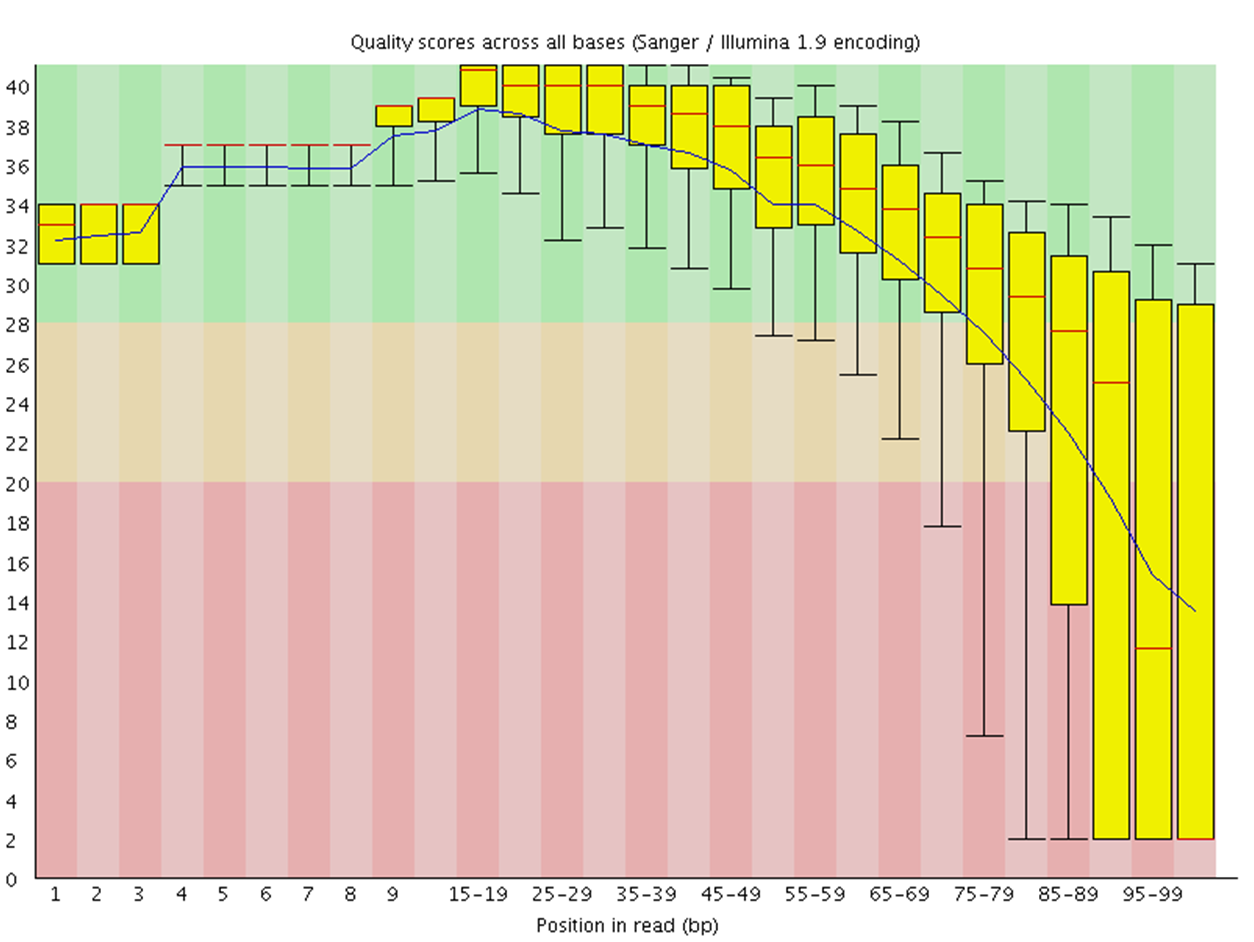
\includegraphics[width=0.8\textwidth]{ngs-qc/bad_example.png}
\caption{Per base sequence quality plot for \texttt{bad\_example.fastq}. Base positions in the reads are shown on x-axis and quality score (Q Score) are shown on the Y-axis}
\label{fig:bad_example_plot}
\end{figure}

\begin{information}
A quality score (or Q-score) expresses an error probability.  In particular, it
serves as a convenient and compact way to communicate very small error
probabilities.
Given an assertion, A, the probability that A is not true, $P(~ A)$, is expressed
by a quality score, $Q(A)$, according to the relationship:
\\\\
$Q(A) =-10 log10(P(\sim A))$
\\\\
Where $P(~ A)$ is the estimated probability of an assertion A being wrong.
The relationship between the quality score and error probability is demonstrated
with the following table:

% Table generated by Excel2LaTeX from sheet 'Sheet1'
\begin{table}[H]
  \centering
  \caption{Error probabilities associated with various quality (Q) values}
    \begin{tabular}{rr}
    \toprule
    \textbf{Quality score, Q(A)} & \textbf{Error probability, P($\sim$A)} \\
    \midrule
    10    & 0.1 \\
    20    & 0.01 \\
    30    & 0.001 \\
    40    & 0.0001 \\
    \bottomrule
    \end{tabular}%
  \label{tab:addlabel}%
\end{table}%

\end{information}

\begin{questions}
How many sequences were there in your file? What is the read length?
\begin{answer}
40,000. read length=100bp
\end{answer}

Does the quality score values vary throughout the read length?
(hint: look at the 'per base sequence quality plot')
\begin{answer}
Yes. Quality scores are dropping towards the end of the reads.
\end{answer}

What is the quality score range you see?
\begin{answer}
2-40
\end{answer}

At around which position do the scores start falling below Q20? 
\begin{answer}
Around 80 bp position
\end{answer}


How can we trim the reads to filter out the low quality data?
\begin{answer}
By trimming off the bases after a fixed position of the read. or by trimming off bases based on the quality score.
\end{answer}
\end{questions}

\begin{bonus}
\subsection{Good Quality Data}
View the FastQC report files fastqc\_report.html to see examples of a good
quality data and compare the quality plot with that of the bad\_example\_fastqc.

\begin{lstlisting}
firefox good_example_fastqc/fastqc_report.html &
\end{lstlisting}
\end{bonus}

\begin{note}
Sequencing errors can complicate the downstream analysis, which normally
requires that reads be aligned to each other (for genome assembly) or to a
reference genome (for detection of mutations). Sequence reads containing errors
may lead to ambiguous paths in the assembly or improper gaps. In variant
analysis projects sequence reads are aligned against the reference genome. The
errors in the reads may lead to more mismatches than expected from
mutations alone. But if these errors can be removed or corrected, the read
alignments and hence the variant detection will improve. The assemblies will also
improve after pre-processing the reads with errors.
\end{note}

\section{Read Trimming}
Read trimming can be done in a variety of different ways. Choose a method
which best suits your data. Here we are giving examples of fixed-length trimming
and quality-based trimming.

\subsection{Fixed Length Trimming}
Low quality read ends can be trimmed using a fixed-length timmer. We will use the
\texttt{fastx\_trimmer} from the FASTX-Toolkit. Usage message to find out various options
you can use with this tool. Type \fonttt{fastx\_trimmer -h} at anytime to display help.

\begin{steps}
We will no do fixed-length trimming of the \texttt{bad\_example.fastq} file
using the following command.
\begin{lstlisting}
cd ~/QC
fastx_trimmer -h
fastx_trimmer -Q 33 -f 1 -l 80 -i bad_example.fastq -o bad_example_trimmed01.fastq
\end{lstlisting}
\end{steps}

\begin{note}
We used the following options in the command above:
\begin{description}[style=multiline,labelindent=0cm,align=right,leftmargin=\descriptionlabelspace,rightmargin=1.5cm,font=\ttfamily]
 \item[-Q 33] Indicates the input quality scores are Phred+33 encoded
 \item[-f] First base to be retianed in the output
 \item[-l] Last base to be retained in the output
 \item[-i] Input fastq file name
 \item[-o] Output file name
\end{description}
\end{note}

\begin{steps}
Run FastQC on the trimmed file and visualise the quality scores of the trimmed file.
\begin{lstlisting}
fastqc -f fastq bad_example_trimmed01.fastq
firefox bad_example_trimmed01_fastqc/fastqc_report.html &
\end{lstlisting}

The output should look like:

\begin{table}[H]
  \centering
  \caption{FastQC Basic Statistics table}
    \begin{tabular}{ll}
    \toprule
    Filename & bad\_example\_trimmed01.fastq\\
    \midrule
    File type & Conventional base calls\\
    Encoding & Sanger / Illumina 1.9\\
    Total Sequences & 40000\\
    Filtered Sequences & 0\\
    Sequence length & 80\\
    \%GC & 48\\
    \bottomrule
    \end{tabular}%
  \label{tab:badexampletrimmed}%
\end{table}%

\begin{figure}[H]
\centering
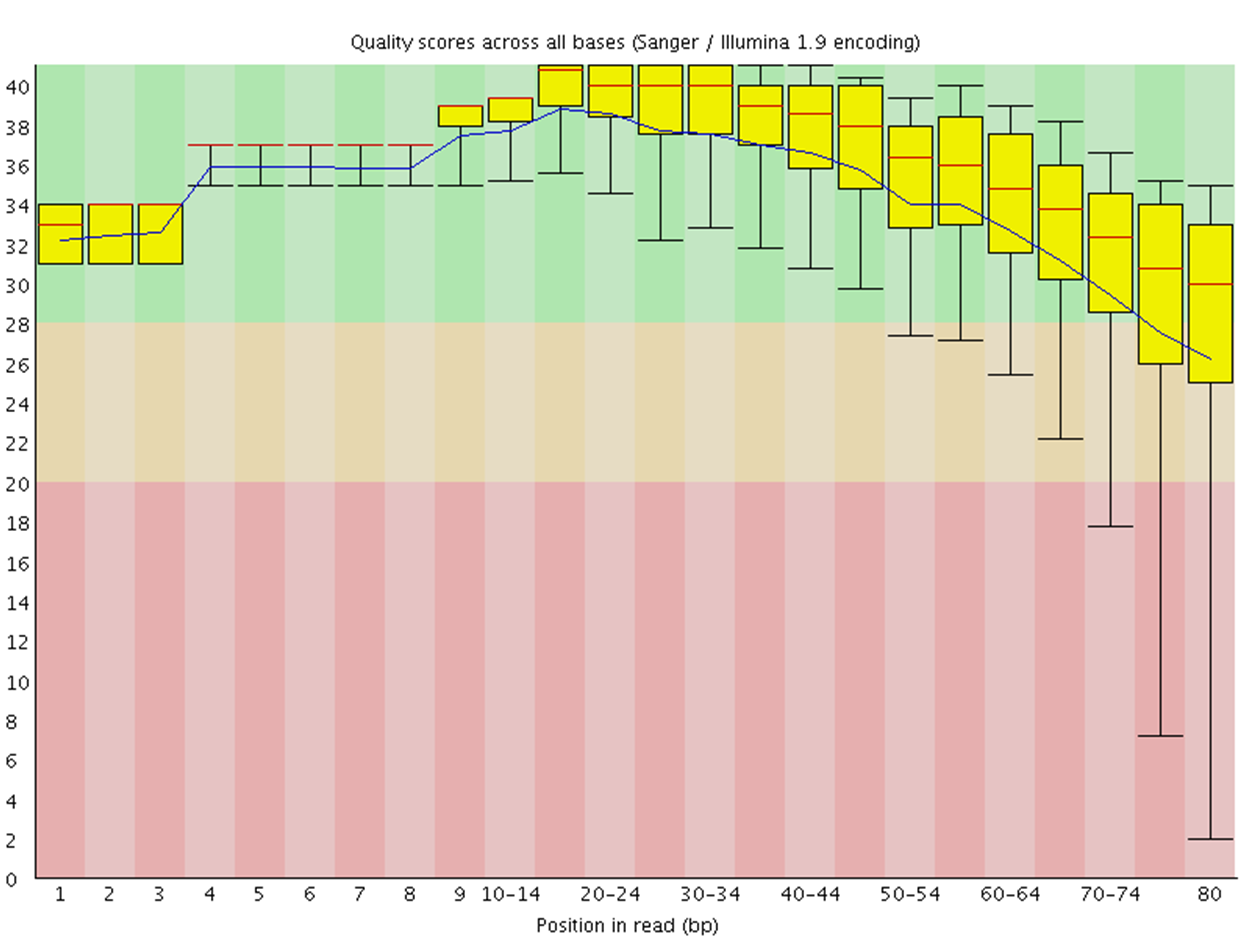
\includegraphics[width=0.8\textwidth]{ngs-qc/bad_example_trimmed_to_80bp.png}
\caption{Per base sequence quality plot for the fixed-length trimmed \texttt{bad\_example.fastq} reads. Base positions in the reads are shown on x-axis and quality score (Q Score) are shown on the Y-axis}
\label{fig:bad_example_trimmed_plot}
\end{figure}

\end{steps}

\begin{questions}
What values would you use for \texttt{-f} if you wanted to trim off 10 bases at
the 5' end of the reads?
\begin{answer}
\texttt{-f 11}
\end{answer}
\end{questions}

\subsection{Quality Based Trimming}
Base call quality scores can also be used to dynamically determine the trim points for each read. A quality
score threshold and minimum read length following trimming can be used to remove low
quality data.

\begin{steps}
Run the following command to quality trim your data:
\begin{lstlisting}
cd ~/QC
fastq_quality_trimmer -h
fastq_quality_trimmer -Q 33 -t 20 -l 50 -i bad_example.fastq -o bad_example_quality_trimmed.fastq
\end{lstlisting}
\end{steps}

\begin{steps}
Run FastQC on the quality trimmed file and visualise the quality scores.

\begin{lstlisting}
fastqc -f fastq bad_example_quality_trimmed.fastq
firefox bad_example_quality_trimmed_fastqc/fastqc_report.html &
\end{lstlisting}

The output should look like:

\begin{table}[H]
  \centering
  \caption{FastQC Basic Statistics table}
    \begin{tabular}{ll}
    \toprule
    Filename & bad\_example\_quality\_trimmed.fastq\\
    \midrule
    File type & Conventional base calls\\
    Encoding & Sanger / Illumina 1.9\\
    Total Sequences & 38976\\
    Filtered Sequences & 0\\
    Sequence length & 50-100\\
    \%GC & 48\\
    \bottomrule
    \end{tabular}%
  \label{tab:badexamplequalitytrimmed}%
\end{table}%

\begin{figure}[H]
\centering
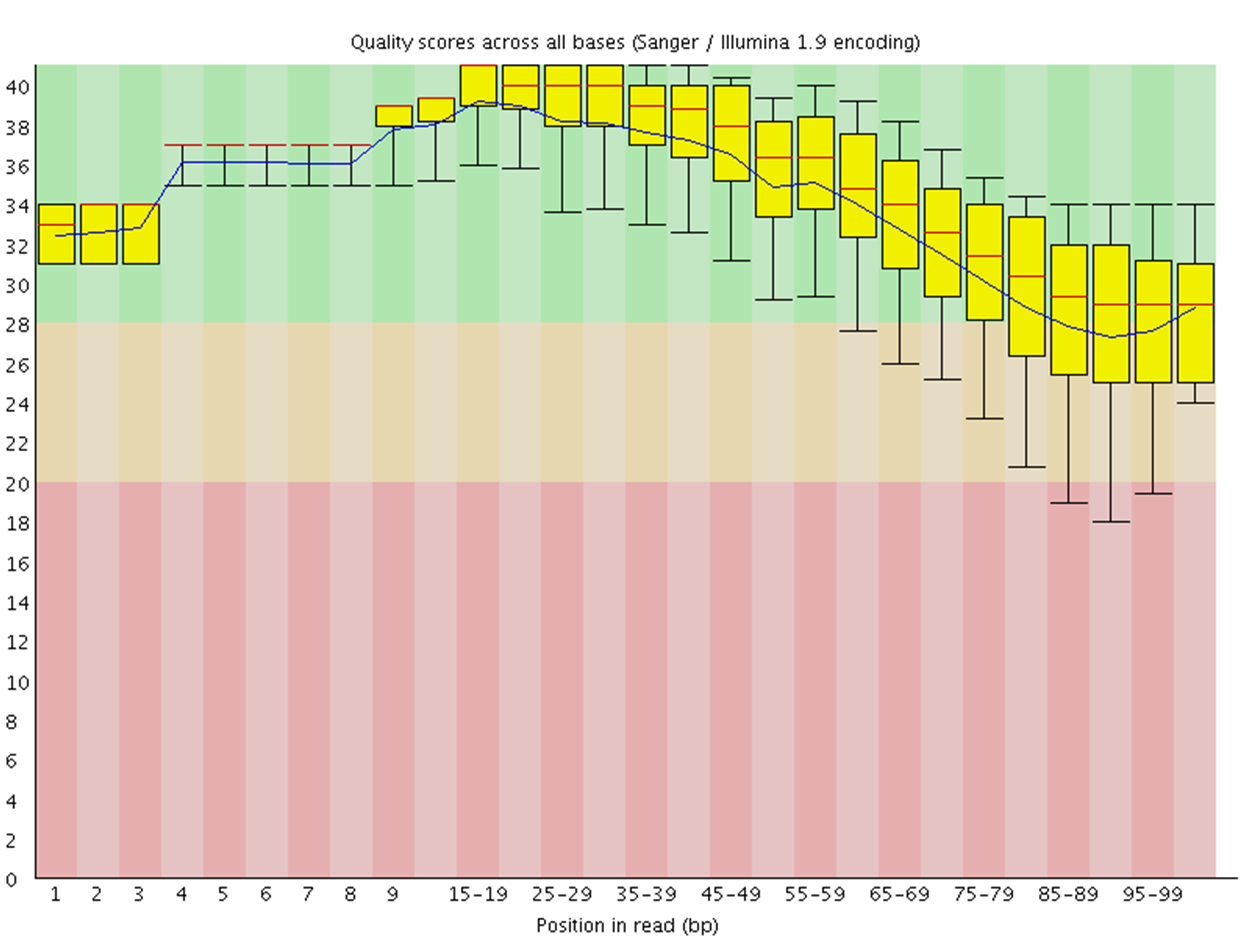
\includegraphics[width=0.8\textwidth]{ngs-qc/bad_example_quality_trimmed.png}
\caption{Per base sequence quality plot for the quality-trimmed \texttt{bad\_example.fastq} reads. Base positions in the reads are shown on x-axis and quality score (Q Score) are shown on the Y-axis}
\label{fig:bad_example_quality_trimmed_plot}
\end{figure}

\end{steps}

\begin{questions}
How did the quality score range change with two types of trimming?
\begin{answer}
Some poor quality bases (Q $<$20) are still present at the 3' end of the
fixed-length trimmed reads. It also removes bases that are good quality.

Quality-based trimming retains the 3' ends of reads which have good quality
scores.
\end{answer}

Did the number of total reads change after two types of trimming?
\begin{answer}
Quality trimming discarded $>$1000 reads. However, We retain a lot of maximal
length reads which have good quality all the way to the ends.
\end{answer}

What reads lengths were obtained after quality based trimming?
\begin{answer}
50-100

Reads $<$50 bp, following quality trimming, were discarded.
\end{answer}

Did you observe adapter sequences in the data?
\begin{answer}
No. (Hint: look at the overrepresented sequences.
\end{answer}

\end{questions}

\begin{advanced}
\subsection{Adapter Clipping}
Sometime sequence reads may end up getting the leftover of adapters and primers
used in the sequencing process. It's good practice to screen your data for
these possible contaminations for more sensitive alignment and assembly based
analysis.

\begin{note}
This is particularly important when read lengths can be longer than the
molecules being sequenced. For example when sequencing miRNAs.
\end{note}

Various QC tools are available to screen and/or clip these adapter/primer
sequences from your data. (e.g. FastQC, fastx, cutadapt).

\begin{steps}
Here we are demonstrating \texttt{fastx\_clipper} to trim a given adapter
sequence.

\begin{lstlisting}
cd ~/QC
fastx_clipper -h
fastx_clipper -v -Q 33 -l 20 -M 15 -a GATCGGAAGAGCGGTTCAGCAGGAATGCCGAG -i bad_example.fastq -o bad_example_clipped.fastq
\end{lstlisting}
\end{steps}

\begin{note}
An alternative tool, not installed on this system, for adapter clipping is
\texttt{fastq-mcf}. A list of adapters is provided in a text file. For more
information, see Fastqmcf at \url{http://code.google.com/p/ea-utils/wiki/FastqMcf}.
\end{note}

\subsection{Removing Duplicates}
Duplicate reads are the ones having the same start and end coordinates. This
may be the result of technical duplication (too many PCR cycles), or
over-sequencing (very high fold coverage). It is very important to put the
duplication level in context of your experiment. For example, duplication level
in targeted or re-sequencing projects may mean something different in RNA-seq
experiments. In RNA-seq experiments oversequencing is usually necessary when
detecting low abundance transcripts.

\begin{information}
The duplication level computed by FastQC is based on sequence identity at the
end of reads. Another tool, Picard, determines duplicates based on identical
start and end positions in SAM/BAM alignment files.

\textbf{We will not cover Picard but
provide the following for your information.}

Picard is a suite of tools for performing many common tasks with SAM/BAM format
files. For more information see the Picard website and information about the
various command-line tools available:

\url{http://picard.sourceforge.net/command-line-overview.shtml}
\end{information}

\begin{information}
Picard 1.69 is installed on this system in \texttt{/usr/share/java/picard-1.69/}

One of the Picard tools (MarkDuplicates) can be used to analyse and remove
duplicates from the raw sequence data. The input for Picard is a sorted
alignment file in BAM format. Short read aligners such as, bowtie, BWA and tophat
can be used to align FASTQ files against a reference genome to generate
SAM/BAM alignment format.
\end{information}

\begin{steps}
Interested users can use the following general command to run the
MarkDuplicates tool at their leisure and only need to provide a BAM file for
INPUT:


\begin{lstlisting}
cd ~/QC
java -jar /usr/share/java/picard/MarkDuplicates.jar INPUT=<alignment_file.bam> VALIDATION_STRINGENCY=LENIENT OUTPUT=alignment_file.dup METRICS_FILE=alignment_file.matric ASSUME_SORTED=true REMOVE_DUPLICATES=true

\end{lstlisting}
\end{steps}

\end{advanced}


%
% Alignment Module
%
% Define the top matter
\renewcommand{\moduleTitle}{Read Alignment}
\renewcommand{\moduleAuthors}{%
  Myrto Kostadima \mailto{kostadim@ebi.ac.uk}
} \renewcommand{\moduleContributions}{%
  Xi Li \mailto{sean.li@csiro.au}%
}

%  Start: Module Title Page
\chapter{\moduleTitle}
\newpage
% End: Module Title Page

\section{Key Learning Outcomes}

After completing this practical the trainee should be able to:
%TODO
\begin{itemize}
  \item Perform the simple NGS data alignment task against one interested reference data \\
  \item Interpret and manipulate the mapping output using samtools \\
  \item Visualise the alignment via a standard genome browser, e.g. IGV browser \\
\end{itemize}
\section{Resources You'll be Using}
 
\subsection{Tools Used}
\begin{description}[style=multiline,labelindent=0cm,align=left,leftmargin=0.5cm]
  \item[Bowtie]\hfill\\
  	\url{http://bowtie-bio.sourceforge.net/index.shtml}
  \item[Bowtie 2]\hfill\\
  	\url{http://bowtie-bio.sourceforge.net/bowtie2/index.shtml}
  \item[Samtools]\hfill\\
  	\url{http://picard.sourceforge.net/}
  \item[BEDTools]\hfill\\
  	\url{http://code.google.com/p/bedtools/}
  \item[UCSC tools]\hfill\\
  	\url{http://hgdownload.cse.ucsc.edu/admin/exe/}  
  \item[IGV genome browser]\hfill\\
  	\url{http://www.broadinstitute.org/igv/}
\end{description}

\subsection{Sources of Data}
  \url{http://www.ebi.ac.uk/arrayexpress/experiments/E-GEOD-11431}
% \url{http://www.ebi.ac.uk/ena/data/view/ERR022484}\\
% \url{http://www.ebi.ac.uk/ena/data/view/ERR022485}

\clearpage

\section{Introduction}

\begin{information}
The goal of this hands-on session is to perform an unspliced alignment for a
small subset of raw reads. We will align raw sequencing data to the mouse genome
using \emph{Bowtie} and then we will manipulate the SAM output in order to
visualize the alignment on the \emph{IGV browser}.
\end{information}

\section{Prepare the Environment}

\begin{information}
We will use one data set in this practical, which can be found in the \texttt{ChIP-seq}
directory on your desktop.
\end{information}

\begin{steps}
Open the Terminal.

First, go to the right folder, where the data are stored.
\begin{lstlisting}
cd ~/ChIP-seq
\end{lstlisting}

\begin{information}
The \texttt{.fastq} file that we will align is called \texttt{Oct4.fastq}. This
file is based on Oct4 ChIP-seq data published by Chen et al. (2008). For the
sake of time, we will align these reads to a single mouse chromosome.
\end{information}
\end{steps}

\section{Alignment}

\begin{information}
You already know that there are a number of competing tools for short read
alignment, each with its own set of strengths, weaknesses, and caveats. Here we
will try \emph{Bowtie}, a widely used ultrafast, memory efficient short read
aligner.
\end{information}

\begin{steps}
\emph{Bowtie} has a number of parameters in order to perform the alignment. To
view them all type

\begin{lstlisting}
bowtie --help
\end{lstlisting}

\emph{Bowtie} uses indexed genome for the alignment in order to keep its memory
footprint small. Because of time constraints we will build the index only for
one chromosome of the mouse genome. For this we need the chromosome sequence in
FASTA format. This is stored in a file named \texttt{mm9}, under the subdirectory
\texttt{bowtie\_index}.

The indexed chromosome is generated using the command:

\begin{lstlisting}
bowtie-build bowtie_index/mm9.fa bowtie_index/mm9
\end{lstlisting}

This command will output 6 files that constitute the index. These files that
have the prefix \texttt{mm9} are stored in the \texttt{bowtie\_index}
subdirectory. To view if they files have been successfully created type:

\begin{lstlisting}
ls -l bowtie_index
\end{lstlisting}
\end{steps}

\begin{information}
Now that the genome is indexed we can move on to the actual alignment. The first
argument for bowtie is the basename of the index for the genome to be searched;
in our case is \texttt{mm9}. We also want to make sure that the output is in SAM
format using the \texttt{-S} parameter. The last argument is the name of the
FASTQ file.
\end{information}

\begin{steps}
Align the Oct4 reads using Bowtie: 

\begin{lstlisting}
bowtie bowtie_index/mm9 -S Oct4.fastq > Oct4.sam
\end{lstlisting}

The above command outputs the alignment in SAM format and stores them in the
file \texttt{Oct4.sam}.
\end{steps}

\begin{note}
In general before you run \emph{Bowtie}, you have to know which encoding your FASTQ files
have. The available FASTQ encodings for bowtie are:

\begin{description}[style=multiline,labelindent=0cm,align=right,leftmargin=\descriptionlabelspace,rightmargin=1.5cm,font=\ttfamily]
 \item[--phred33-quals] Input quals are Phred+33 (default).
 \item[--phred64-quals] Input quals are Phred+64 (same as \texttt{--solexa1.3-quals}).
 \item[--solexa-quals] Input quals are from GA Pipeline ver. $<$ 1.3.
 \item[--solexa1.3-quals] Input quals are from GA Pipeline ver. $\geq$ 1.3.
 \item[--integer-quals] Qualities are given as space-separated integers (not ASCII).
\end{description}

The FASTQ files we are working with are Sanger encoded (Phred+33), which is the
default for \emph{Bowtie}.

\emph{Bowtie} will take 2-3 minutes to align the file. This is fast compared to
other aligners which sacrifice some speed to obtain higher sensitivity.
\end{note}

\begin{steps}
Look at SAM format by typing:

\begin{lstlisting}
head -n 10 Oct4.sam
\end{lstlisting}
\end{steps}

\begin{questions}
Can you distinguish between the header of the SAM format and the actual alignments?
\begin{answer}
%TODO
The header line starts with the letter `@', i.e.: 

\begin{tabular}{llll}
@HD & VN:1.0 & SO:unsorted & \\
@SQ & SN:chr1 & LN:197195432 & \\
@PG & ID:Bowtie &      VN:0.12.8  & CL:``bowtie bowtie\_index/mm9 -S Oct4.fastq'' \\
\end{tabular}

While, the actual alignments start with read id, i.e.:

\begin{tabular}{llll}
SRR002012.45 & 0 & chr1 & etc \\
SRR002012.48 & 16 & chr1 & etc \\
\end{tabular}
\end{answer}

What kind of information does the header provide?
\begin{answer}
%TODO
1. @HD: Header line; VN: Format version; SO: the sorting order of alignment.
2. @SQ: Reference sequence information; SN: reference sequence name; LN: reference sequence length.
3. @PG: Read group information; ID: Read group identifier; VN: Program version; CL: the command line that produces the alignment.
\end{answer}

To which chromosome are the reads mapped? 
\begin{answer}
%TODO
Chromosome 1.
\end{answer}
\end{questions}

\section{Manipulate SAM output}

\begin{note}
SAM files are rather big and when dealing with a high volume of NGS data,
storage space can become an issue. As we have already seen, we can convert SAM
to BAM files (their binary equivalent that are not human readable) that occupy
much less space.
\end{note}

\begin{steps}
Convert SAM to BAM using \emph{samtools} and store the output in the file
\texttt{Oct4.bam}. You have to instruct \emph{samtools} that the input is in SAM
format (\texttt{-S}), the output should be in BAM format (\texttt{-b}) and that
you want the output to be stored in the file specified by the \texttt{-o}
option:

\begin{lstlisting}
samtools view -bSo Oct4.bam Oct4.sam
\end{lstlisting}
\end{steps}

\begin{advanced}
Compute simple stats of the alignment using \emph{samtools}:

\begin{lstlisting}
samtools flagstat Oct4.bam
\end{lstlisting}
\end{advanced}

\section{Visualize alignments in IGV}

\begin{information}
\emph{IGV} is a stand-alone genome browser. Please check their website
(\url{http://www.broadinstitute.org/igv/}) for all the formats that \emph{IGV}
can display. For our visualization purposes we will use the BAM and bigWig
formats.
\end{information}

\begin{note}
When uploading a BAM file into the genome browser, the browser will look for the
index of the BAM file in the same folder where the BAM files is. The index file
should have the same name as the BAM file and the suffix \texttt{.bai}. Finally, to
create the index of a BAM file you need to make sure that the file is sorted
according to chromosomal coordinates.
\end{note}

\begin{steps}
Sort alignments according to chromosome position and store the result in the
file with the prefix \texttt{Oct4.sorted}:

\begin{lstlisting}
samtools sort Oct4.bam Oct4.sorted
\end{lstlisting}

Index the sorted file.

\begin{lstlisting}
samtools index Oct4.sorted.bam
\end{lstlisting}

The indexing will create a file called \texttt{Oct4.sorted.bam.bai}. Note that
you don't have to specify the name of the index file when running samtools.
\end{steps}

\begin{note}
Another way to visualize the alignments is to convert the BAM file into a bigWig
file. The bigWig format is for display of dense, continuous data and the data
will be displayed as a graph. The resulting bigWig files are in an indexed
binary format.
\end{note}

\begin{steps}
The BAM to bigWig conversion takes place in two steps. Firstly, we convert the
BAM file into a bedgraph, called \texttt{Oct4.bedgraph}, using the tool
\texttt{genomeCoverageBed} from \emph{BEDTools}:

\begin{lstlisting}
genomeCoverageBed -bg -ibam Oct4.sorted.bam -g bowtie_index/mouse.mm9.genome > Oct4.bedgraph
\end{lstlisting}

Then we convert the bedgraph into a binary graph, called \texttt{Oct4.bw}, using the
tool \texttt{bedGraphToBigWig} from the \emph{UCSC} tools:

\begin{lstlisting}
bedGraphToBigWig Oct4.bedgraph bowtie_index/mouse.mm9.genome Oct4.bw
\end{lstlisting}
\end{steps}

\begin{note}
Both of the commands above take as input a file called \texttt{mouse.mm9.genome} that
is stored under the subdirectory \texttt{bowtie\_index}. These genome files are
tab-delimited and describe the size of the chromosomes for the organism of
interest. When using the UCSC Genome Browser, Ensembl, or Galaxy, you typically
indicate which species/genome build you are working. The way you do this for
\emph{BEDTools} is to create a ``genome'' file, which simply lists the names of
the chromosomes (or scaffolds, etc.) and their size (in basepairs).

\emph{BEDTools} includes pre-defined genome files for human and mouse in the
\texttt{genomes} subdirectory included in the \emph{BEDTools} distribution.
\end{note}

\begin{steps}
Now we will load the data into the IGV browser for visualization. In order to
launch IGV double click on the IGV 2.1 icon on your Desktop. Ignore any warnings
and when it opens you have to load the genome of interest.

On the top left of your screen choose from the drop down menu \texttt{Mus musculus
(mm9)}. Then in order to load the desire files go to:

\begin{lstlisting}
File > Load from File
\end{lstlisting}

On the pop up window navigate to Desktop $>$ ChIP-seq folder and select the file
\texttt{Oct4.sorted.bam}.

Repeat these steps in order to load \texttt{Oct4.bw} as well.

Select chr1 from the drop down menu on the top left. Right click on the name of
\texttt{Oct4.bw} and choose Maximum under the Windowing Function. Right click again and
select Autoscale.

In order to see the aligned reads of the BAM file, you need to zoom in to a
specific region. For example, look for gene \texttt{Lemd1} in the search box.
\end{steps}

\begin{questions}
What is the main difference between the visualization of BAM and bigWig files?
\begin{answer}
%TODO
The actual alignment of reads that stack to a particular region can be displayed using the information stored in a BAM format.
The bigWig format is for display of dense, continuous data that will be displayed in the Genome Browser as a graph.
\end{answer}
\end{questions}

Using the \texttt{+} button on the top right zoom in more to see the details of the alignment.

\begin{questions}
What do you think the different colors mean?
\begin{answer}
%TODO
The different color represents four nucleotides, e.g. blue is Cytidine (C), red is Thymidine (T).
\end{answer}
\end{questions}

\section{Practice}
In the ChIP-seq folder you will find another \texttt{.fastq} file called
\texttt{gfp.fastq}. Follow the above described analysis for this dataset as well.



%
% ChIP-Seq Module
%
% Define the top matter
\renewcommand{\moduleTitle}{ChIP-Seq}
\renewcommand{\moduleAuthors}{%
  Remco Loos, EMBL-EBI \mailto{remco@ebi.ac.uk} \\
  Myrto Kostadima \mailto{kostadim@ebi.ac.uk}
} \renewcommand{\moduleContributions}{%
  Xi Li \mailto{sean.li@csiro.au}%
}

%  Start: Module Title Page
\chapter{\moduleTitle}
\newpage
% End: Module Title Page

\section{Key Learning Outcomes}

After completing this practical the trainee should be able to:
\begin{itemize}
  \item Perform simple ChIP-Seq analysis, e.g. the detection of immuno-enriched areas using the chosen peak caller program MACS
  \item Visualize the peak regions through a genome browser, e.g. Ensembl, and identify the real peak regions
  \item Perform functional annotation and detect potential binding sites (motif) in the predicted binding regions using motif discovery tool, e.g. MEME.
\end{itemize}

\section{Resources You'll be Using}
 
\subsection{Tools Used}
\begin{description}[style=multiline,labelindent=0cm,align=left,leftmargin=0.5cm]
  \item[MACS]\hfill\\
  	\url{http://liulab.dfci.harvard.edu/MACS/index.html}
  \item[Ensembl]\hfill\\
  	\url{http://www.ensembl.org}
  \item[PeakAnalyzer]\hfill\\
  	\url{http://www.ebi.ac.uk/bertone/software}
  \item[MEME]\hfill\\
  	\url{http://meme.ebi.edu.au/meme/cgi-bin/meme.cgi}
  \item[TOMTOM]\hfill\\
  	\url{http://meme.ebi.edu/meme/cgi-bin/tomtom.cgi}  
  \item[DAVID]\hfill\\
  	\url{http://david.abcc.ncifcrf.gov}
  \item[GOstat]\hfill\\
    \url{http://gostat.wehi.edu.au}
\end{description}

\subsection{Sources of Data}
  \url{http://www.ebi.ac.uk/arrayexpress/experiments/E-GEOD-11431}
 % These data are reported in Chen, X et al. (2008) Integration of external signaling pathways with the core tran-scriptional network in embryonic stem cells. Cell. Jun 13;133(6):1106-17.


\newpage

\section{Introduction}

\begin{information}
The goal of this hands-on session is to perform some basic tasks in the analysis
of ChIP-seq data. In fact, you already performed the first step, alignment of
the reads to the genome, in the previous session. We start from the aligned
reads and we will find immuno-enriched areas using the peak caller MACS. We will
visualize the identified regions in a genome browser and perform functional
annotation and motif analysis on the predicted binding regions.
\end{information}

\section{Prepare the Environment}

\begin{information}
The material for this practical can be found in the \texttt{ChIP-seq} directory on your
desktop. This directory also contains an electronic version of this document,
which can be useful to copy and paste commands. Please make sure that this
directory also contains the SAM/BAM files you produced during the alignment
practical.
\end{information}

\begin{steps}
If you didn't have time to align the control file called \texttt{gfp.fastq}
during the alignment practical, please do it now. Follow the same steps, from
the bowtie alignment step, as for the \texttt{Oct4.fastq} file.
\end{steps}

\begin{note}
In ChIP-seq analysis (unlike in other applications such as RNA-seq) it can be useful
to exclude all reads that map to more than one location in the
genome. When using Bowtie, this can be done using the
\texttt{-m 1} option, which tells it to report only unique matches (See
\texttt{bowtie --help} for more details).
\end{note}


\begin{steps}
Open the Terminal and go to the \texttt{ChIP-seq} directory:
\begin{lstlisting}
cd ~/ChIP-seq
\end{lstlisting}
\end{steps}

\section{Finding enriched areas using MACS}

\begin{information}
MACS stands for Model based analysis of ChIP-seq. It was designed for
identifying transcription factor binding sites. MACS captures the influence of
genome complexity to evaluate the significance of enriched ChIP regions, and
improves the spatial resolution of binding sites through combining the
information of both sequencing tag position and orientation. MACS can be easily
used for ChIP-Seq data alone, or with a control sample to increase specificity.
\end{information}

\begin{steps}
Consult the MACS help file to see the options and parameters:

\begin{lstlisting}
macs --help
\end{lstlisting}
\end{steps}

\begin{information}
The input for MACS can be in ELAND, BED, SAM, BAM or BOWTIE formats (you just
have to set the \texttt{--format} option).

Options that you will have to use include: 

\begin{description}[style=multiline,labelindent=0cm,align=right,leftmargin=\descriptionlabelspace,rightmargin=1.5cm,font=\ttfamily]
 \item[-t] To indicate the input ChIP file.
 \item[-c] To indicate the name of the control file.
 \item[--format] To change the file format. The default format is bed.
 \item[--name] To set the name of the output files.
 \item[--gsize] This is the mappable genome size. With the read length we have,
 $70\%$ of the genome is a fair estimation. Since in this analysis we include
 only reads from chromosome 1 (197Mbases), we will use a \texttt{--gsize} of 138Mbases (70\% of 197Mbases).
 \item[--tsize] To set the read length (look at the FASTQ files to check the
 length).
 \item[--wig] To generate signal wig files for viewing in a genome browser.
 Since this process is time consuming, it is recommended to run MACS first with
 this flag off, and once you decide on the values of the parameters, run MACS
 again with this flag on.
 \item[--diag] To generate a saturation table, which gives an indication whether
 the sequenced reads give a reliable representation of the possible peaks.
\end{description}
\end{information}

\begin{steps}
Now run macs using the following command:

\begin{lstlisting}
macs -t <Oct4_aligned_bam_file> -c <gfp_aligned_bam_file> --format=BAM --name=Oct4 --gsize=138000000 --tsize=26 --diag --wig 
\end{lstlisting}

Look at the output saturation table (\texttt{Oct4\_diag.xls}). To open this file
file, right-click on it and choose ``Open with'' and select LibreOffice. Do you think
that more sequencing is necessary?

Open the Excel peak file and view the peak details. Note that the number of tags
(column 6) refers to the number of reads in the whole peak region and not the
peak height.

\end{steps}

\section{Viewing results with the Ensembl genome browser}

\begin{information}
It is often instructive to look at your data in a genome browser. Before, we
used IGV, a stand-alone browser, which has the advantage of being installed
locally and providing fast access. Web-based genome browsers, like Ensembl or
the UCSC browser, are slower, but provide more functionality. They do not only
allow for more polished and flexible visualisation, but also provide easy access
to a wealth of annotations and external data sources. This makes it
straightforward to relate your data with information about repeat regions, known
genes, epigenetic features or areas of cross-species conservation, to name just
a few. As such, they are useful tools for exploratory analysis.

They will allow you to get a `feel' for the data, as well as detecting
abnormalities and problems. Also, exploring the data in such a way may give you
ideas for further analyses.
\end{information}

\begin{steps}
Launch a web browser and go to the Ensembl website at
\url{http://www.ensembl.org/index.html}

Choose the genome of interest (in this case, mouse) on the left side of the
page, browse to any location in the genome or click one of the demo links
provided on the web page.

Click on the \textbf{Manage your data} link on the left, then choose
\textbf{Attach remote file}.

\end{steps}

\begin{note}
Wig files are large so are inconvenient for uploading directly to the Ensemble Genome browser. Instead, we will convert it to an indexed binary format
and put this into a web accessible place such as on a HTTP, HTTPS, or FTP server.
This makes all the browsing process much faster. Detailed
instructions for generating a bigWig from a wig type file can be found at:

\url{http://genome.ucsc.edu/goldenPath/help/bigWig.html}.

\end{note}

\begin{steps}
We have generated bigWig files in advance for you to upload to the Ensembl
browser. They are at the following URL:
\url{http://www.ebi.ac.uk/~remco/ChIP-Seq_course/Oct4.bw}

To visualise the data:
\begin{itemize}
	\item Paste the location above in the field File URL. 
	\item Choose data format bigWig. 
	\item Choose some informative name and in the next window choose the colour of your preference. 
	\item Click \textbf{Save} and close the window to return to the genome browser. 
\end{itemize}
Repeat the process for the gfp control sample, located at
\url{http://www.ebi.ac.uk/~remco/ChIP-Seq_course/gfp.bw}.
 
After uploading, choose \textbf{Configure this page}, and under \textbf{Your
data} tick both boxes. Closing the window will save these changes.

Go to a region on chromosome 1 (e.g. \texttt{1:34823162-35323161}), and zoom in and out
to view the signal and peak regions. Be aware that the y-axis of each track is auto-scaled independently of each other,
so bigger-looking peaks may not actually be bigger! Always look at the values
on the left hand side axis.
\end{steps}

\begin{questions}
What can you say about the profile of Oct4 peaks in this region? 
\begin{answer}
There are no significant Oct4 peaks over the selected region.
\end{answer}

Compare it with H3K4me3 histone modification wig file we have generated at 
\url{http://www.ebi.ac.uk/~remco/ChIP-Seq_course/H3K4me3.bw}. 
\begin{answer}
H3K4me3 has a region that contains relatively high peaks than Oct4. 
\end{answer}

Jump to \texttt{1:36066594-36079728} for a sample peak. Do you think H3K4me3
peaks regions contain one or more modification sites? What about Oct4?
\begin{answer}
Yes. There are roughly three peaks, which indicate the possibility of having more than one modification sites in this region. 

For Oct4, no peak can be observed.
\end{answer}

\end{questions}

\begin{note}
MACS generates its peak files in a file format called bed file. This is a simple
text format containing genomic locations, specified by chromosome, begin and end
positions, and some more optional information.

See \url{http://genome.ucsc.edu/FAQ/FAQformat.html#format1} for details.

Bed files can also be uploaded to the Ensembl browser.
\end{note}

\begin{advanced}
Try uploading the peak file generated by MACS to Ensembl. Find the first peak in
the file (use the \texttt{head} command to view the beginning of the bed file), and see
if the peak looks convincing to you.
\end{advanced}


\section{Annotation: From peaks to biological interpretation}

\begin{information}
In order to biologically interpret the results of ChIP-seq experiments, it is
usually recommended to look at the genes and other annotated elements that are
located in proximity to the identified enriched regions. This can be easily done
using PeakAnalyzer.
\end{information}

\begin{steps}
Go to the PeakAnalyzer directory and launch the program by typing:
\begin{lstlisting}
cd ~ChIP-seq/PeakAnalyzer
java -jar PeakAnalyzer.jar &
\end{lstlisting}

The first window allows you to choose between the split application (which we
will try next) and peak annotation. Choose the peak annotation option and click
\textbf{Next}.

We would like to find the closest downstream genes to each peak, and the genes
that overlap with the peak region. For that purpose you should choose the
\textbf{NDG} option and click \textbf{Next}.

Fill in the location of the peak file \texttt{Oct4\_peaks.bed}, and choose the mouse GTF
as the annotation file. You don't have to define a symbol file since gene
symbols are included in the GTF file.

Choose the output directory and run the program.
\end{steps}

\begin{information}
When the program has finished running, you will have the option to generate
plots, by pressing the \textbf{Generate plots} button. This is only possible if R is
installed on your computer, as it is on this system. A PDF file with the plots will be generated in
the output folder. You could generate similar plots with Excel using the output files that
were generated by PeakAnalyzer. 
\end{information}

\begin{note}
This list of closest downstream genes (contained in the file
\texttt{Oct4\_peaks.ndg.bed}) can be the basis of further analysis. For instance,
you could look at the Gene Ontology terms associated with these genes to get an
idea of the biological processes that may be affected. Web-based tools like
DAVID (\url{http://david.abcc.ncifcrf.gov}) or GOstat
(\url{http://gostat.wehi.edu.au}) take a list of genes and return the enriched
GO categories.
\end{note}

\begin{bonus}
We can pull out Ensemble Transcript IDs from the \texttt{Oct4\_peaks.ndg.bed}
file and write them to another file ready for use with DAVID or GOstat:
\begin{lstlisting}
cut -f 5 Oct4_peaks.ndg.bed | sed '1 d' > Oct4_peaks.ndg.tid
\end{lstlisting}
\end{bonus}

\section{Motif analysis}

\begin{information}
It is often interesting to find out whether we can associate identified the
binding sites with a sequence pattern or motif. We will use MEME for motif
analysis. The input for MEME should be a file in FASTA format containing the
sequences of interest. In our case, these are the sequences of the identified
peaks that probably contain Oct4 binding sites.

Since many peak-finding tools merge overlapping areas of enrichment, the
resulting peaks tend to be much wider than the actual binding sites.
Sub-dividing the enriched areas by accurately partitioning enriched loci into a
finer-resolution set of individual binding sites, and fetching sequences from
the summit region where binding motifs are most likely to appear enhances the
quality of the motif analysis. Sub-peak summit sequences can be retrieved
directly from the Ensembl database using PeakAnalyzer.
\end{information}

\begin{steps}
If you have closed the PeakAnalyzer running window, open it again. If it is
still open, just go back to the first window.

Choose the split peaks utility and click \textbf{Next}. The input consists of
files generated by most peak-finding tools: a file containing the chromosome,
start and end locations of the enriched regions, and a \texttt{.wig} signal file
describing the size and shape of each peak. Fill in the location of both files
\texttt{Oct4\_peaks.bed} and the wig file generated by MACS, which is under the
\texttt{Oct4\_MACS\_wiggle/treat/} directory, check the option to \textbf{Fetch subpeak
sequences} and click \textbf{Next}.

In the next window you have to set some parameters for splitting the peaks.

\begin{description}[style=multiline,labelindent=0cm,align=right,leftmargin=\descriptionlabelspace,rightmargin=1.5cm,font=\ttfamily]
 \item[Separation float] Keep the default value. This value determines when a
 peak will be separated into sub-peaks. This is the ratio between a valley and
 its neighbouring summit (the lower summit of the two). For example, if you set
 this height to be \texttt{0.5}, two sub-peaks will be separated only if the
 height of the lower summit is twice the height of the valley.
 \item[Minimum height] Set this to be \texttt{5}. Only sub-peaks with at least this
 number of tags in their summit region will be separated. Change the organism
 name from the default human to mouse and run the program.
\end{description}
\end{steps}

\begin{information}
Since the program has to read large wig files, it will take a few minutes to
run. Once the run is finished, two output files will be produced. The first
describes the location of the sub-peaks, and the second is a FASTA file
containing 300 sequences of length 61 bases, taken from the summit regions of
the highest sub-peaks.
\end{information}

\begin{steps}
Open a web bowser and go to the MEME website at
\url{http://meme.ebi.edu.au/meme/cgi-bin/meme.cgi}, and fill in the necessary
details, such as:
\begin{itemize}
	\item Your e-mail address 
	\item The sub-peaks FASTA file \texttt{Oct4\_peaks.bestSubPeaks.fa} (will need uploading), or just paste in the sequences. 
	\item The number of motifs we expect to find (1 per sequence) 
	\item The width of the desired motif (between 6 to 20) 
	\item The maximum number of motifs to find (3 by default). For Oct4 one classical motif is known. 
\end{itemize}
\end{steps}

\begin{note}
You will receive the results by e-mail. This usually doesn't take more than a few minutes.
\end{note}

\begin{steps}
Open the e-mail and click on the link that leads to the HTML results page.

Scroll down until you see the first motif logo. We would like to know if this
motif is similar to any other known motif. We will use TOMTOM for this. Scroll
down until you see the option \textbf{Submit this motif to}. Click the TOMTOM
button to compare to known motifs in motif databases, and on the new page choose
to compare your motif to those in the JASPAR and UniPROBE database.
\end{steps}


\begin{questions}
Which motif was found to be the most similar to your motif?
\begin{answer}
Sox2
\end{answer}
\end{questions}

\newpage
\section{Reference}
%TODO Use BibTeX
Chen, X et al.: Integration of external signaling pathways with the core transcriptional network in embryonic stem cells. Cell 133:6, 1106-17 (2008).


%
% RNA-Seq Module
%
% Define the top matter
\setModuleTitle{RNA-Seq}
\setModuleAuthors{%
  Myrto Kostadima, EMBL-EBI \mailto{kostadmi@ebi.ac.uk}\\
  Remco Loos, EMBL-EBI \mailto{remco@ebi.ac.uk}
}
\setModuleContributions{%
  Nathan S. Watson-Haigh \mailto{nathan.watson-haigh@awri.com.au}%
}

%  Start: Module Title Page
\chapter{\moduleTitle}
\newpage
% End: Module Title Page

\section{Key Learning Outcomes}

After completing this practical the trainee should be able to:
\begin{itemize}
  \item Understand and perform a simple RNA-Seq analysis workflow.
  \item Perform gapped alignments to an indexed reference genome using TopHat.
  \item Perform transcript assembly using Cufflinks.
  \item Visualize transcript alignments and annotation in a genome browser such as IGV.
  \item Be able to identify differential gene expression between two experimental conditions.
\end{itemize}

\section{Resources You'll be Using}
 
\subsection{Tools Used}
\begin{description}[style=multiline,labelindent=0cm,align=left,leftmargin=1cm]
  \item[Tophat] \hfill\\
    \url{http://tophat.cbcb.umd.edu/}
  \item[Cufflinks] \hfill\\
    \url{http://cufflinks.cbcb.umd.edu/}
  \item[Samtools] \hfill\\
    \url{http://samtools.sourceforge.net/}
  \item[BEDTools] \hfill\\
    \url{http://code.google.com/p/bedtools/}
  \item[UCSC tools] \hfill\\
    \url{http://hgdownload.cse.ucsc.edu/admin/exe/}
  \item[IGV] \hfill\\
    \url{http://www.broadinstitute.org/igv/}
  \item[DAVID Functional Analysis] \hfill\\
    \url{http://david.abcc.ncifcrf.gov/}
\end{description}

\subsection{Sources of Data}
\url{http://www.ebi.ac.uk/ena/data/view/ERR022484}\\
\url{http://www.ebi.ac.uk/ena/data/view/ERR022485}

\newpage

\section{Introduction}
The goal of this hands-on session is to perform some basic tasks in the
downstream analysis of RNA-seq data. We will start from RNA-seq data aligned to
the zebrafish genome using Tophat.

We will perform transcriptome reconstruction using Cufflinks and we will compare
the gene expression between two different conditions in order to identify
differentially expressed genes.

\section{Prepare the Environment}
We will use a dataset derived from sequencing of mRNA from \textit{Danio rerio} embryos
in two different developmental stages. Sequencing was performed on the Illumina
platform and generated 76bp paired-end sequence data using polyA selected RNA.
Due to the time constraints of the practical we will only use a subset of the
reads.

The data files are contained in the subdirectory called \texttt{data} and are
the following:
\begin{description}[style=multiline,labelindent=1.5cm,align=left,leftmargin=2.5cm]
  \item[\texttt{2cells\_1.fastq} and \texttt{2cells\_2.fastq}] \hfill\\
 These files are based on RNA-seq data of a 2-cell zebrafish embryo
  \item[\texttt{6h\_1.fastq} and \texttt{6h\_2.fastq}] \hfill\\
 These files are based on RNA-seq data of zebrafish embryos 6h post
 fertilization
\end{description}

\begin{steps}
Open the Terminal and go to the \texttt{RNA-seq} working directory:
\begin{lstlisting}
cd ~/RNA-seq/
\end{lstlisting}
\end{steps}

%\reversemarginpar\marginpar{\vskip+0em\hfill
\includegraphics[height=1cm]{./graphics/warning.png}}
%\textcolor{red}{
\begin{warning}
  All commands entered into the terminal for this tutorial should be from within the
  \textbf{\texttt{$\sim$/RNA-seq}} directory.
\end{warning}

\begin{steps}
Check that the \texttt{data} directory contains the above-mentioned files by typing:
\begin{lstlisting}
ls data
\end{lstlisting}
\end{steps}

\section{Alignment}
There are numerous tools for performing short read alignment and the choice of aligner
should be carefully made according to the analysis goals/requirements. Here we will
use Tophat, a widely used ultrafast aligner that performs spliced alignments.

Tophat is based on the Bowtie aligner and uses an indexed genome for the
alignment to speed up the alignment and keep its memory footprint small. 
The the index for the \textit{Danio rerio} genome has been created for you. 

\begin{warning}
The commands to create an index follow, do not run
\begin{lstlisting}
bowtie-build genome/Danio_rerio.Zv9.66.dna.fa genome/ZV9
\end{lstlisting}
\end{warning}

\begin{steps}
Tophat has a number of parameters in order to perform the alignment. To view them all type:
\begin{lstlisting}
tophat --help
\end{lstlisting}
\end{steps}

\begin{information}
The general format of the tophat command is:
\begin{lstlisting}[style=command_syntax]
tophat [options]* <index_base> <reads_1> <reads_2>
\end{lstlisting}

Where the last two arguments are the \texttt{.fastq} files of the paired end
reads, and the argument before is the basename of the indexed genome.
\end{information}

\begin{note}
The quality values in the FASTQ files used in this hands-on session are Phred+33
encoded. We explicitly tell tophat of this fact by using the command line
argument \texttt{--solexa-quals}.
\end{note}

\begin{information}
You can look at the first few reads in the file \texttt{data/2cells\_1.fastq} with:
 
\begin{lstlisting}
head -n 20 data/2cells_1.fastq
\end{lstlisting}
\end{information}

%\reversemarginpar\marginpar{\vskip+0em\hfill
\includegraphics[height=1cm]{./graphics/notes.png}}
\begin{note}
Some other parameters that we are going to use to run Tophat are listed below:
\begin{description}[style=multiline,labelindent=0cm,align=right,leftmargin=\descriptionlabelspace,rightmargin=1.5cm,font=\ttfamily]
 \item[-g] Maximum number of multihits allowed. Short reads are likely to map to
 more than one location in the genome even though these reads can have originated
 from only one of these regions. In RNA-seq we allow for a limited number of
 multihits, and in this case we ask Tophat to report only reads that map at most
 onto 2 different loci.
 \item[--library-type] Before performing any type of RNA-seq analysis you need
 to know a few things about the library preparation. Was it done using a
 strand-specific protocol or not? If yes, which strand? In our data the protocol
 was NOT strand specific.
 \item[-j] Improve spliced alignment by providing Tophat with annotated splice
 junctions. Pre-existing genome annotation is an advantage when analysing RNA-seq
 data. This file contains the coordinates of annotated splice junctions from Ensembl.
 These are stored under the sub-directory \texttt{annotation} in a file called
 \texttt{ZV9.spliceSites}.
 \item[-o] This specifies in which subdirectory Tophat should save the output
 files. Given that for every run the name of the output files is the same, we
 specify different directories for each run.
\end{description}
\end{note}

It takes some time (approx. 20 min) to perform tophat spliced alignments, even for this subset of
reads. Therefore, we have pre-aligned the \texttt{2cells} data for you using the following command:
\begin{warning}
You DO NOT need to run this command yourself - we have done this for you.

\begin{lstlisting}
tophat --solexa-quals -g 2 --library-type fr-unstranded -j annotation/Danio_rerio.Zv9.66.spliceSites -o tophat/ZV9_2cells genome/ZV9 data/2cells_1.fastq data/2cells_2.fastq
\end{lstlisting}
\end{warning}

\begin{steps}
Align the \texttt{6h} data yourself using the following command:  

\begin{lstlisting}
# Takes approx. 20mins
tophat --solexa-quals -g 2 --library-type fr-unstranded -j annotation/Danio_rerio.Zv9.66.spliceSites -o tophat/ZV9_6h genome/ZV9 data/6h_1.fastq data/6h_2.fastq
\end{lstlisting}

\end{steps}

The \texttt{6h} read alignment will take approx. 20 min to complete. Therefore,
we'll take a look at some of the files, generated by tophat, for the
pre-computed \texttt{2cells} data.

\subsection{Alignment Visualisation in IGV}

The Integrative Genomics Viewer (IGV) is able to provide a visualisation of read
alignments given a reference sequence and a BAM file. We'll visualise the
information contained in the \texttt{accepted\_hits.bam} and
\texttt{junctions.bed} files for the pre-computed \texttt{2cells} data. The
former, contains the tophat sliced alignments of the reads to the reference
while the latter stores the coordinates of the splice junctions present in the
data set.

\begin{steps}
Open the \texttt{RNA-seq} directory on your Desktop and double-click the
\texttt{tophat} subdirectory and then the \texttt{ZV9\_2cells} directory.

\begin{enumerate}
  \item Launch IGV by double-clicking the ``IGV 2.3'' icon on the Desktop
  (ignore any warnings that you may get as it opens). \emph{NOTE: IGV may take
  several minutes to load for the first time, please be patient.}
  \item Choose ``Zebrafish (Zv9)'' from the drop-down box in the top left of the
  IGV window. Else you can also load the genome fasta file.
  \item Load the \texttt{accepted\_hits.sorted.bam} file by clicking the
  ``File'' menu, selecting ``Load from File'' and navigating to the
  \texttt{Desktop/RNA-seq/tophat/ZV9\_2cells} directory.
  \item Rename the track by right-clicking on its name and choosing ``Rename
  Track''. Give it a meaningful name like ``2cells BAM''.
  \item Load the \texttt{junctions.bed} from the same directory and rename the
  track ``2cells Junctions BED''.
  \item Load the Ensembl annotations file \texttt{Danio\_rerio.Zv9.66.gtf}
  stored in the \texttt{RNA-seq/annotation} directory.
  \item Navigate to a region on chromosome 12 by typing
  \texttt{chr12:20,270,921-20,300,943} into the search box at the top of the IGV
  window.
\end{enumerate}

\end{steps}

\begin{information}
Keep zooming to view the bam file alignments

Some useful IGV manuals can be found below

http://www.broadinstitute.org/software/igv/interpreting_insert_size
http://www.broadinstitute.org/software/igv/alignmentdata
\end{information}


\begin{questions}
Can you identify the splice junctions from the BAM file?
\begin{answer}
Slice junctions can be identified in the alignment BAM files.
These are the aligned RNA-Seq reads that have skipped-bases from the reference genome (most likely introns).
\end{answer}

Are the junctions annotated for \texttt{CBY1} consistent with the annotation?
\begin{answer}
Read alignment supports an extended length in exon 5 to the gene model (cby1-001) 
\end{answer}

Are all annotated genes, from both RefSeq and Ensembl, expressed?
\begin{answer}
No BX000473.1-201 is not expressed
\end{answer}

\end{questions}

\begin{steps}
Once tophat finishes aligning the 6h data you will need to sort the alignments found in the BAM file and then index the
sorted BAM file.

\begin{lstlisting}
samtools sort tophat/ZV9_6h/accepted_hits.bam tophat/ZV9_6h/accepted_hits.sorted
samtools index tophat/ZV9_6h/accepted_hits.sorted.bam
\end{lstlisting}

Load the sorted BAM file into IGV, as described previously, and rename the track appropriately.
\end{steps}

\newpage
\section{Isoform Expression and Transcriptome Assembly}
There are a number of tools that perform reconstruction of the transcriptome
and for this workshop we are going to use Cufflinks. Cufflinks can do
transcriptome assembly either \textit{ab initio} or using a reference annotation. It
also quantifies the isoform expression in Fragments
Per Kilobase of exon per Million fragments mapped (FPKM).

\begin{steps}
Cufflinks has a number of parameters in order to perform transcriptome
assembly and quantification. To view them all type:

\begin{lstlisting}
cufflinks --help
\end{lstlisting}
\end{steps}

We aim to reconstruct the transcriptome for both samples by using the Ensembl
annotation both strictly and as a guide. In the first case Cufflinks will only
report isoforms that are included in the annotation, while in the latter case
it will report novel isoforms as well.

The Ensembl annotation for \textit{Danio rerio} is available in
\texttt{annotation/Danio\_rerio.Zv9.66.gtf}.

\begin{information}
The general format of the \texttt{cufflinks} command is:
\begin{lstlisting}[style=command_syntax]
cufflinks [options]* <aligned_reads.(sam|bam)>
\end{lstlisting}
Where the input is the aligned reads (either in SAM or BAM format).
\end{information}

\begin{note}
Some of the available parameters for Cufflinks that we are going to use to run
Cufflinks are listed below:
\begin{description}[style=multiline,labelindent=0cm,align=right,leftmargin=\descriptionlabelspace,rightmargin=1.5cm,font=\ttfamily]
  \item[-o] Output directory.
  \item[-G] Tells Cufflinks to use the supplied GTF annotations strictly in order
  to estimate isoform annotation.
  \item[-b] Instructs Cufflinks to run a bias detection and correction algorithm
  which can significantly improve accuracy of transcript abundance estimates.
  To do this Cufflinks requires a multi-fasta file with the genomic sequences
  against which we have aligned the reads.
  \item[-u] Tells Cufflinks to do an initial estimation procedure to more
  accurately weight reads mapping to multiple locations in the genome
  (multi-hits).
  \item[--library-type] Before performing any type of RNA-seq analysis you need
  to know a few things about the library preparation. Was it done using a
  strand-specific protocol or not? If yes, which strand? In our data the protocol
  was NOT strand specific.
\end{description}
\end{note}

\begin{steps}
Perform transcriptome assembly, strictly using the supplied GTF annotations, for the \texttt{2cells} and \texttt{6h} data using cufflinks:
\begin{lstlisting}
# 2cells data (takes approx. 5mins):
cufflinks -o cufflinks/ZV9_2cells_gtf -G annotation/Danio_rerio.Zv9.66.gtf -b genome/Danio_rerio.Zv9.66.dna.fa -u --library-type fr-unstranded tophat/ZV9_2cells/accepted_hits.bam
# 6h data (takes approx. 5mins):
cufflinks -o cufflinks/ZV9_6h_gtf -G annotation/Danio_rerio.Zv9.66.gtf -b genome/Danio_rerio.Zv9.66.dna.fa -u --library-type fr-unstranded tophat/ZV9_6h/accepted_hits.bam
\end{lstlisting}
\end{steps}

\begin{information}
Cufflinks generates several files in the specified output directory. Here's a short description of these files:

\begin{description}[style=multiline,labelindent=0cm,align=right,leftmargin=\descriptionlabelspace,rightmargin=1.5cm,font=\ttfamily]
\item[genes.fpkm\_tracking] Contains the estimated gene-level expression values.
\item[isoforms.fpkm\_tracking] Contains the estimated isoform-level expression values.
\item[skipped.gtf] Contains loci skipped as a result of exceeding the maximum number of fragments.
\item[transcripts.gtf] This GTF file contains Cufflinks' assembled isoforms.
\end{description}

The complete documentation can be found at:
\url{http://cufflinks.cbcb.umd.edu/manual.html#cufflinks_output}
\end{information}

\begin{information}
So far we have forced cufflinks, by using the \texttt{-G} option, to strictly
use the GTF annotations provided and thus novel transcripts will not be reported. We
can get cufflinks to perform a GTF-guided transcriptome assembly by using the
\texttt{-g} option instead. Thus, novel transcripts will be reported.

\end{information}

\begin{warning}
GTF-guided transcriptome assembly is more computationally intensive than
strictly using the GTF annotations. Therefore, we have pre-computed these
GTF-guided assemblies for you and have placed the results under subdirectories:
\texttt{cufflinks/ZV9\_2cells\_gtf\_guided} and
\texttt{cufflinks/ZV9\_6h\_gft\_guided}.

You DO NOT need to run these commands. We provide them so you know how we
generated the the GTF-guided transcriptome assemblies:
\begin{lstlisting}
# 2cells guided transcriptome assembly (takes approx. 30mins):
cufflinks -o cufflinks/ZV9_2cells_gtf_guided -g annotation/Danio_rerio.Zv9.66.gtf -b genome/Danio_rerio.Zv9.66.dna.fa -u --library-type fr-unstranded tophat/ZV9_2cells/accepted_hits.bam
# 6h guided transcriptome assembly (takes approx. 30mins):
cufflinks -o cufflinks/ZV9_6h_gtf_guided -g annotation/Danio_rerio.Zv9.66.gtf -b genome/Danio_rerio.Zv9.66.dna.fa -u --library-type fr-unstranded tophat/ZV9_6h/accepted_hits.bam
\end{lstlisting}

\end{warning}

\begin{steps}
\begin{enumerate}
  \item Go back to IGV and load the pre-computed, GTF-guided transcriptome
  assembly for the \texttt{2cells} data
  (\texttt{cufflinks/ZV9\_2cells\_gtf\_guided/transcripts.gtf}).
  \item Rename the track as ``2cells GTF-Guided Transcripts''.
  \item In the search box type \texttt{ENSDART00000082297} in order for the
  browser to zoom in to the gene of interest.
\end{enumerate}
\end{steps}

\begin{questions}
Do you observe any difference between the Ensembl GTF annotations and the
GTF-guided transcripts assembled by cufflinks (the ``2cells GTF-Guided Transcripts'' track)?
\begin{answer}
Yes. It appears that the Ensembl annotations may have truncated the last exon.
However, our data also doesn't contain reads that span between the last two
exons.
\end{answer}

\end{questions}

\section{Differential Expression}
One of the stand-alone tools that perform differential expression analysis is
Cuffdiff. We use this tool to compare between two conditions; for example
different conditions could be control and disease, or wild-type and mutant, or
various developmental stages.

In our case we want to identify genes that are
differentially expressed between two developmental stages; a \texttt{2cells}
embryo and \texttt{6h} post fertilization.

\begin{information}
The general format of the cuffdiff command is:
\begin{lstlisting}[style=command_syntax]
cuffdiff [options]* <transcripts.gtf> <sample1_replicate1.sam[,...,sample1_replicateM]> <sample2_replicate1.sam[,...,sample2_replicateM.sam]>
\end{lstlisting}

Where the input includes a \texttt{transcripts.gtf} file, which is an annotation
file of the genome of interest, and the aligned reads (either in SAM or BAM
format) for the conditions.
Some of the Cufflinks options that we will use to run the program are:
\begin{description}[style=multiline,labelindent=0cm,align=right,leftmargin=\descriptionlabelspace,rightmargin=1.5cm,font=\ttfamily]
  \item[-o] Output directory.
  \item[-L] Labels for the different conditions
  \item[-T] Tells Cuffdiff that the reads are from a time series experiment.
  \item[-b] Instructs Cufflinks to run a bias detection and correction algorithm
  which can significantly improve accuracy of transcript abundance estimates.
  To do this Cufflinks requires a multi-fasta file with the genomic sequences
  against which we have aligned the reads.
  \item[-u] Tells Cufflinks to do an initial estimation procedure to more
  accurately weight reads mapping to multiple locations in the genome
  (multi-hits). 
  \item[--library-type] Before performing any type of RNA-seq analysis you need
 to know a few things about the library preparation. Was it done using a
 strand-specific protocol or not? If yes, which strand? In our data the protocol
 was NOT strand specific.
\end{description}
\end{information}

\begin{steps}
Run cuffdiff on the cufflinks generated BAM files for the 2cells vs. 6h data sets:
\begin{lstlisting}
cuffdiff -o cuffdiff/ -L ZV9_2cells,ZV9_6h -T -b genome/Danio_rerio.Zv9.66.dna.fa -u --library-type fr-unstranded annotation/Danio_rerio.Zv9.66.gtf tophat/ZV9_2cells/accepted_hits.bam tophat/ZV9_6h/accepted_hits.bam
\end{lstlisting}
\end{steps}

\begin{steps}
We are interested in the differential expression at the gene level. The results
are reported by Cuffdiff in the file \texttt{cuffdiff/gene\_exp.diff}. 
Look at the first few lines of the file using the following command:
\begin{lstlisting}
head -n 20 cuffdiff/gene_exp.diff
\end{lstlisting}

We would like to see which are the most significantly differentially expressed
genes. Therefore we will sort the above file according to the q value
(corrected p value for multiple testing). The result will be stored in a
different file called \texttt{gene\_exp\_qval.sorted.diff}.
\begin{lstlisting}
sort -t$'\t' -g -k 13 cuffdiff/gene_exp.diff > cuffdiff/gene_exp_qval.sorted.diff
\end{lstlisting}

Look again at the first few lines of the sorted file by typing:
\begin{lstlisting}
head -n 20 cuffdiff/gene_exp_qval.sorted.diff
\end{lstlisting}

Copy an Ensembl transcript identifier from the first two columns for one of
these genes (e.g. \texttt{ENSDARG00000077178}). Now go back to the IGV browser
and paste it in the search box.
\end{steps}

\begin{questions}
Do you see any difference in the read coverage between the \texttt{2cells} and
\texttt{6h} conditions that might have given rise to this transcript being
called as differentially expressed?
\begin{warning}
Note that the coverage on the Ensembl browser is based on raw reads and no
normalisation has taken place contrary to the FPKM values.
\end{warning}

\begin{answer}
The read coverage of this transcript (\texttt{ENSDARG00000077178}) in the 2cells
data set is much higher than in the 6h data set.
\end{answer}

\end{questions}

\begin{bonus}
\section{Functional Annotation of Differentially Expressed Genes}
After you have performed the differential expression analysis you are interested
in identifying if there is any functionality enrichment for your differentially
expressed genes.
On your Desktop click:
\begin{lstlisting}[style=command_syntax]
Applications >> Internet >> Firefox Web Browser
\end{lstlisting}
And go to the following URL: \url{http://david.abcc.ncifcrf.gov/}
On the left side click on Functional Annotation. Then click on the Upload tab.
Under the section Choose from File, click Choose File and navigate to the
\texttt{cuffdiff} directory. Select the file called \texttt{globalDiffExprs\_Genes\_qval.01\_top100.tab}.
Under Step 2 select ENSEMBL\_GENE\_ID from the drop-down menu. Finally select
Gene list and then press Submit List.
Click on Gene Ontology and then click on the CHART button of the GOTERM\_BP\_ALL item.

\begin{questions}
Do these categories make sense given the samples we're studying?
\begin{answer}
Developmental Biology
\end{answer}

Browse around DAVID website and check what other information are available.
\begin{answer}
Cellular component, Molecular function, Biological Processes, Tissue expression, Pathways, Literature, Protein domains 
\end{answer}
\end{questions}
\end{bonus}

\newpage

\section{References}
%TODO Change to using BiBTeX
\begin{enumerate}
  \item Trapnell, C., Pachter, L. \& Salzberg, S. L. TopHat: discovering splice
  junctions with RNA-Seq. Bioinformatics 25, 1105-1111 (2009).
  \item Trapnell, C. et al. Transcript assembly and quantification by RNA-Seq
  reveals unannotated transcripts and isoform switching during cell
  differentiation. Nat. Biotechnol. 28, 511-515 (2010).
  \item Langmead, B., Trapnell, C., Pop, M. \& Salzberg, S. L. Ultrafast and
  memory-efficient alignment of short DNA sequences to the human genome.
  Genome Biol. 10, R25 (2009).
  \item Roberts, A., Pimentel, H., Trapnell, C. \& Pachter, L. Identification
  of novel transcripts in annotated genomes using RNA-Seq. Bioinformatics 27,
  2325-2329 (2011).
  \item Roberts, A., Trapnell, C., Donaghey, J., Rinn, J. L. \& Pachter, L.
  Improving RNA-Seq expression estimates by correcting for fragment bias.
  Genome Biol. 12, R22 (2011).
\end{enumerate}


%
% Velvet de novo assembly
%
% Define the top matter
\renewcommand{\moduleTitle}{\textit{de novo} Assembly}
\renewcommand{\moduleAuthors}{%
  Matthias Haimel \mailto{mhaimel@ebi.ac.uk}\\
  Nathan S. Watson-Haigh \mailto{nathan.watson-haigh@awri.com.au}
} \renewcommand{\moduleContributions}{%
  
}

%  Start: Module Title Page
\chapterstyle{module}
\chapter{\moduleTitle}
\newpage
% End: Module Title Page

\section{Key Learning Outcomes}

TODO

\section{Resources You'll be Using}
Although we have provided you with an environment which contains all the tools
and data you will be using in this module, you may like to know where we have
sourced those tools and data from.
 
\subsection{Tools Used}
\begin{description}[style=multiline,labelindent=0cm,align=left,leftmargin=1cm]
  \item[Velvet] \hfill\\
  	\url{http://www.ebi.ac.uk/~zerbino/velvet/}
  \item[AMOS Hawkeye] \hfill\\
    \url{http://apps.sourceforge.net/mediawiki/amos/index.php?title=Hawkeye}
  \item[gnx-tools] \hfill\\
    \url{https://github.com/mh11/gnx-tools}
  \item[FastQC] \hfill\\
    \url{http://www.bioinformatics.bbsrc.ac.uk/projects/fastqc/}
  \item[R] \hfill\\
    \url{http://www.r-project.org/}
\end{description}

\subsection{Sources of Data}
\begin{itemize}
\item \url{http://www.ebi.ac.uk/ena/data/view/SRS004748}
\item \url{ftp://ftp.sra.ebi.ac.uk/vol1/fastq/SRR022/SRR022825/SRR022825.fastq.gz}
\item \url{ftp://ftp.sra.ebi.ac.uk/vol1/fastq/SRR022/SRR022823/SRR022823.fastq.gz}
\item \url{http://www.ebi.ac.uk/ena/data/view/SRS004748}
\item \url{ftp://ftp.ensemblgenomes.org/pub/release-8/bacteria/fasta/Staphylococcus/s_aureus_mrsa252/dna/s_aureus_mrsa252.EB1_s_aureus_mrsa252.dna.chromosome.Chromosome.fa.gz}
\item \url{ftp://ftp.sra.ebi.ac.uk/vol1/fastq/SRR022/SRR022852/SRR022852_1.fastq.gz}
\item \url{ftp://ftp.sra.ebi.ac.uk/vol1/fastq/SRR022/SRR022852/SRR022852_2.fastq.gz}
\item \url{ftp://ftp.sra.ebi.ac.uk/vol1/fastq/SRR023/SRR023408/SRR023408_1.fastq.gz}
\item \url{ftp://ftp.sra.ebi.ac.uk/vol1/fastq/SRR023/SRR023408/SRR023408_2.fastq.gz}
\item \url{ftp://ftp.sra.ebi.ac.uk/vol1/fastq/SRR000/SRR000892/SRR000892.fastq.gz}
\item \url{ftp://ftp.sra.ebi.ac.uk/vol1/fastq/SRR000/SRR000893/SRR000893.fastq.gz}
\item \url{http://www.ebi.ac.uk/ena/data/view/SRX007709}
\item \url{http://www.ebi.ac.uk/ena/data/view/SRX000181}
\end{itemize}

\newpage

\section{Introduction}
Some general introduction

\section{Prepare the Environment}
\begin{information}
The first exercise should get you comfortable with the computer environment. I
am going to assume that either you have some minimal experience with command
line UNIX, or that the very short introduction I should have given you by now
was sufficient. Please ask if neither of the above is true. It is not as tricky
as it looks \ldots honest!
\end{information}

\begin{steps}
First make sure that you are in your home directory by typing:
\begin{lstlisting}
cd
\end{lstlisting}

and making absolutely sure you're there by typing:
\begin{lstlisting}
pwd
\end{lstlisting}

Now create sub-directories for this and the two other velvet practicals. All
these directories will be made as sub-directories of a directory for the whole
course called NGS. For this you can use the following commands:
\begin{lstlisting}
mkdir -p NGS/velvet/{part1,part2,part3}
\end{lstlisting}
\end{steps}

\begin{information}
The \texttt{-p} tells \texttt{mkdir} (make directory) to make any parent
directories if they don't exist. You could create the directories one-at-a-time
by doing:
\begin{lstlisting}
mkdir NGS
mkdir NGS/velvet
mkdir NGS/velvet/part1
mkdir NGS/velvet/part2
mkdir NGS/velvet/part3
\end{lstlisting}
\end{information}

\begin{steps}
After creating the directories, examine the structure and move into the
directory ready for the first velvet exercise by typing:
\begin{lstlisting}
ls -R NGS
cd NGS/velvet/part1
pwd
\end{lstlisting}

\end{steps}

\section{Downloading and Compiling Velvet}
\begin{note}
For the duration of this workshop, all the software you require has been set up
for you already. This might not be the case when you return to �real life�. Many
of the programs you will need, including velvet, are quite easy to set up, it
might be instructive to try a couple.
\end{note}

\begin{information}
Although you will be using the preinstalled version of velvet, it is useful to
know how to compile velvet as some of the parameters you might like to control
can only be set at compile time. You can find the latest version of velvet at:

\center{\url{http://www.ebi.ac.uk/~zerbino/velvet/}}

You could go to this URL and download the latest velvet version, or
equivalently, you could type the following, which will download, unpack,
inspect, compile and execute your locally compiled version of velvet:
\begin{lstlisting}
cd ~/NGS/velvet/part1
pwd
cp ~/NGS/Data/velvet_1.2.07.tgz ./
tar xzf ~/NGS/Data/velvet_1.2.07.tgz
ls -R
cd velvet_1.2.07
make velveth velvetg
./velveth
\end{lstlisting}
\end{information}

\begin{steps}
Take a look at the executables you have created. They will be displayed as green
by the command:
\begin{lstlisting}
ls --color=always
\end{lstlisting}
\end{steps}

\begin{notes}
The switch \texttt{--color}, offensively misspelled in American!, instructs that
files be coloured according to their type. This is often the default. Here we
are just being cautious. The \texttt{=always} is included as colouring is
usually suppressed in scripts. If you run this exercise using the script
provided, just \texttt{--color} would not be enough. \texttt{--color=always}
insists on file colouring even from a script.
\end{notes}

\begin{steps}
Have a look of the output the command produces and you will see that
\texttt{MAXKMERLENGTH=31} and \texttt{CATEGORIES=2} parameters were passed into
the compiler.

This indicates that the default compilation was set for De Bruijn graph k-mers of
maximum size 31 and to allow a maximum of just 2 read categories. You can
override these, and other, default configuration choices using command line
parameters. Assume, you want to run velvet with a k-mer length of 41 using 3
categories, velvet needs to be recompiled to enable this functionality by
typing:
\begin{lstlisting}
make clean
make velveth velvetg MAXKMERLENGTH=41 CATEGORIES=3;
./velveth
\end{lstlisting}
\end{steps}

\begin{questions}
Discuss with the persons next to you the following questions:

What are the consequences of the parameters you have given make for velvet?
\begin{answer}
MAXKMERLENGTH: increase the max kmer length from 31 to 41

CATEGORIES: paired-end data require to be put into separate categories. By
increasing this parameter from 2 to 3 allows you to process 3 paired / mate-pair
libraries and unpaired data.
\end{answer}

Why does Velvet use k-mer 31 and 2 categories as default?
\begin{answer}
Possibly a number of reason:\\
  - odd number to avoid palindromes\\
  - The first reads were very short (20-40 bp) and there were hardly any paired-end data\\
     around so there was no need to allow for longer kmer lengths / more categories.\\
  - For programmers: 31 bp get stored in 64 bits (using 2bit encoding)
\end{answer}

Should you get better results by using a longer k-mer length?
\begin{answer}
If you can achieve a good kmer coverage - yes.
\end{answer}
\end{questions}

\begin{steps}
velvet can also be used to process SOLID colour space data. To do this you need
a further make parameter. With the following command clean away your last
compilation and try the following parameters:
\begin{lstlisting}
make clean
make MAXKMERLENGTH=41 CATEGORIES=3 color
./velveth_de
\end{lstlisting}

\end{steps}

\begin{questions}
What effect would the following compil-time parameters have on velvet:\\
\texttt{OPENMP=Y}

\texttt{LONGSEQUENCES=Y}

\texttt{BIGASSEMBLY=Y}

\texttt{VBIGASSEMBLY=Y}

\texttt{SINGLE\_COV\_CAT=Y}

\end{questions}

\begin{notes}
For a further description of velvet compile and runtime parameters please see
the velvet Manual: \url{https://github.com/dzerbino/velvet/wiki/Manual}
\end{notes}

\newpage
\section{Assembling Single-end Reads}

\begin{notes}
The data you will examine is from Staphylococcus aureus USA300 which has a
genome of around 3MB . The reads are Illumina and are unpaired, also known as
single-end library. Even though you have carefully installed velvet in your own
workspace, we will use a pre-installed version.

The data needed for this section can be obtained from the Sequence Read Archive
(SRA). For the following example use the run data SRR022825 and SRR022823 from
the SRA Sample SRS004748. The SRA experiment could be viewed by setting your
browser to the URL:

\center{\url{http://www.ebi.ac.uk/ena/data/view/SRS004748}}

\begin{warning}
We have already downloaded the data files for you.
\end{lstlisting}

\end{warning}
\end{notes}

\begin{information}
The following exercise focuses on velvet using single-end reads, how the
available parameters effect an assembly and how to measure and compare the
changes.
\end{information}

\begin{steps}
To begin with, first move back to the directory you prepared for this exercise,
create a new folder with a suitable name for this part and move into it. There
is no need to download1 the read files, as they are already stored locally.
Instead we will create soft links to the files. Continue by copying (or typing):
\begin{lstlisting}
cd ~/NGS/velvet/part1
mkdir SRS004748
cd SRS004748
pwd
ln -s ~/NGS/Data/SRR022825.fastq.gz ./
ln -s ~/NGS/Data/SRR022823.fastq.gz ./
ls -l
\end{lstlisting}
\end{steps}

\begin{information}
You are ready to process your data with velvet, which is a compressed fastq file.
Velvet has two main components:
\begin{description}[style=multiline,labelindent=1cm,align=left,leftmargin=2cm]
  \item[velveth] \hfill\\
    Used to construct, from raw read data, a dataset organised in the
    fashion expected by the   second component, velvetg.
  \item[velvetg] \hfill\\
    The core of velvet where the de Bruijn graph assembly is built and
    manipulated.
\end{description}

You can always get further information about the usage of both velvet programs
by typing \texttt{velvetg} or \texttt{velveth} in your terminal.
\end{information}

\begin{steps}
Now run velveth for the reads in \texttt{SRR022825.fastq.gz} and
\texttt{SRR022823.fastq.gz} using the following options:
\begin{itemize}
  \item A de Bruijn graph k-mer of 25
  \item An output directory called run\_25
\end{itemize}
\begin{lstlisting}
velveth run_25 25 -fastq.gz -short SRR022825.fastq.gz SRR022823.fastq.gz
\end{lstlisting}

\texttt{velveth} talks to itself for a while and ends with some files in the
output directory. Move into the output directory \texttt{run\_25} and take a look
around at what \texttt{velveth} had done so far. The UNIX command \texttt{less}
allows you to look at output files (press \texttt{q} for quit). Just in case you
still need a hint:

\begin{lstlisting}
cd run_25
ls -l
head Sequences
cat Log
\end{lstlisting}

\end{steps}

\begin{questions}
What did you find in the folder \texttt{run\_25}?

\vspace{2cm}

Describe the content of the two \texttt{velveth} output files?

\vspace{2cm}

What does the \texttt{Log} file store for you?

\vspace{2cm}
\end{questions}

\begin{steps}
Now move one directory level up and run velvetg on your output directory, with
the commands:
\begin{lstlisting}
cd ../
time velvetg run_25
\end{lstlisting}

Move back into your results directory to examine the effects of velvetg:
\begin{lstlisting}
cd run_22
ls -l
\end{lstlisting}

\begin{questions}
What extra files do you see in the folder \texttt{run\_25}?

\vspace{2cm}

What do you suppose they might represent?

\vspace{2cm}
  
In the Log file in \texttt{run\_25}, what is the N50?

\vspace{2cm}

\end{questions}

\begin{information}
Hopefully, we will have discussed what the N50 statistic is by this point.
Broadly, it is the median (not average) of a sorted data set using the length of
a set of sequences. Usually it is the length of the contig whose length, when
added to the length of all longer contigs, makes a total greater that half the
sum of the lengths of all contigs. Easy, but messy � a more formal definition
can be found here:

\center{\url{http://www.broadinstitute.org/crd/wiki/index.php/N50}}
\end{information}

\begin{steps}
Backup the \texttt{contigs.fa} file and calculate the N50 (and the N25,N75) value with
the command:
\begin{lstlisting}
cp contigs.fa contigs.fa.0
gnx -min 100 -nx 25,50,75 contigs.fa
\end{lstlisting}

\end{steps}

\begin{questions}
Does the value of N50 agree with the value stored in the Log file?

\vspace{2cm}

If not, why do you think this might be?

\vspace{2cm}

\end{questions}

\begin{information}
In order to improve our results, take a closer look at the standard options of
\texttt{velvetg} by typing \texttt{velvetg} without parameters. For the moment
focus on the two options \texttt{-cov\_cutoff} and \texttt{-exp\_cov}. Clearly
\texttt{-cov\_cutoff} will allow you to exclude contigs for which the k-mer
coverage is low, implying unacceptably poor quality.
The \texttt{-exp\_cov} switch is used to give \texttt{velvetg} an idea of the
coverage to expect.

If the expected coverage of any contig is substantially in excess of the
suggested expected value, maybe this would indicate a repeat. For further
details of how to choose the parameters, go to 'Choice of a coverage cutoff':

\center{\url{http://wiki.github.com/dzerbino/velvet/}}

\end{information}

\begin{steps}
Briefly, the k-mer coverage (and much more information) for each contig is stored
in the file \texttt{stats.txt} and can be used with R to visualize the coverage
distribution. Take a look at the \texttt{stats.txt} file, start R, load and
visualize the data using the following commands:
\begin{lstlisting}
R --no-save --no-restore
library(plotrix)
data <- read.table("stats.txt", header=TRUE)
weighted.hist(data$short1_cov, data$lgth, breaks=0:50)
\end{lstlisting}

A weighted histogram is a better way of visualizing the coverage information,
because of noise (lots of very short contigs). You can see an example output
below:

\begin{figure}[H]
\centering
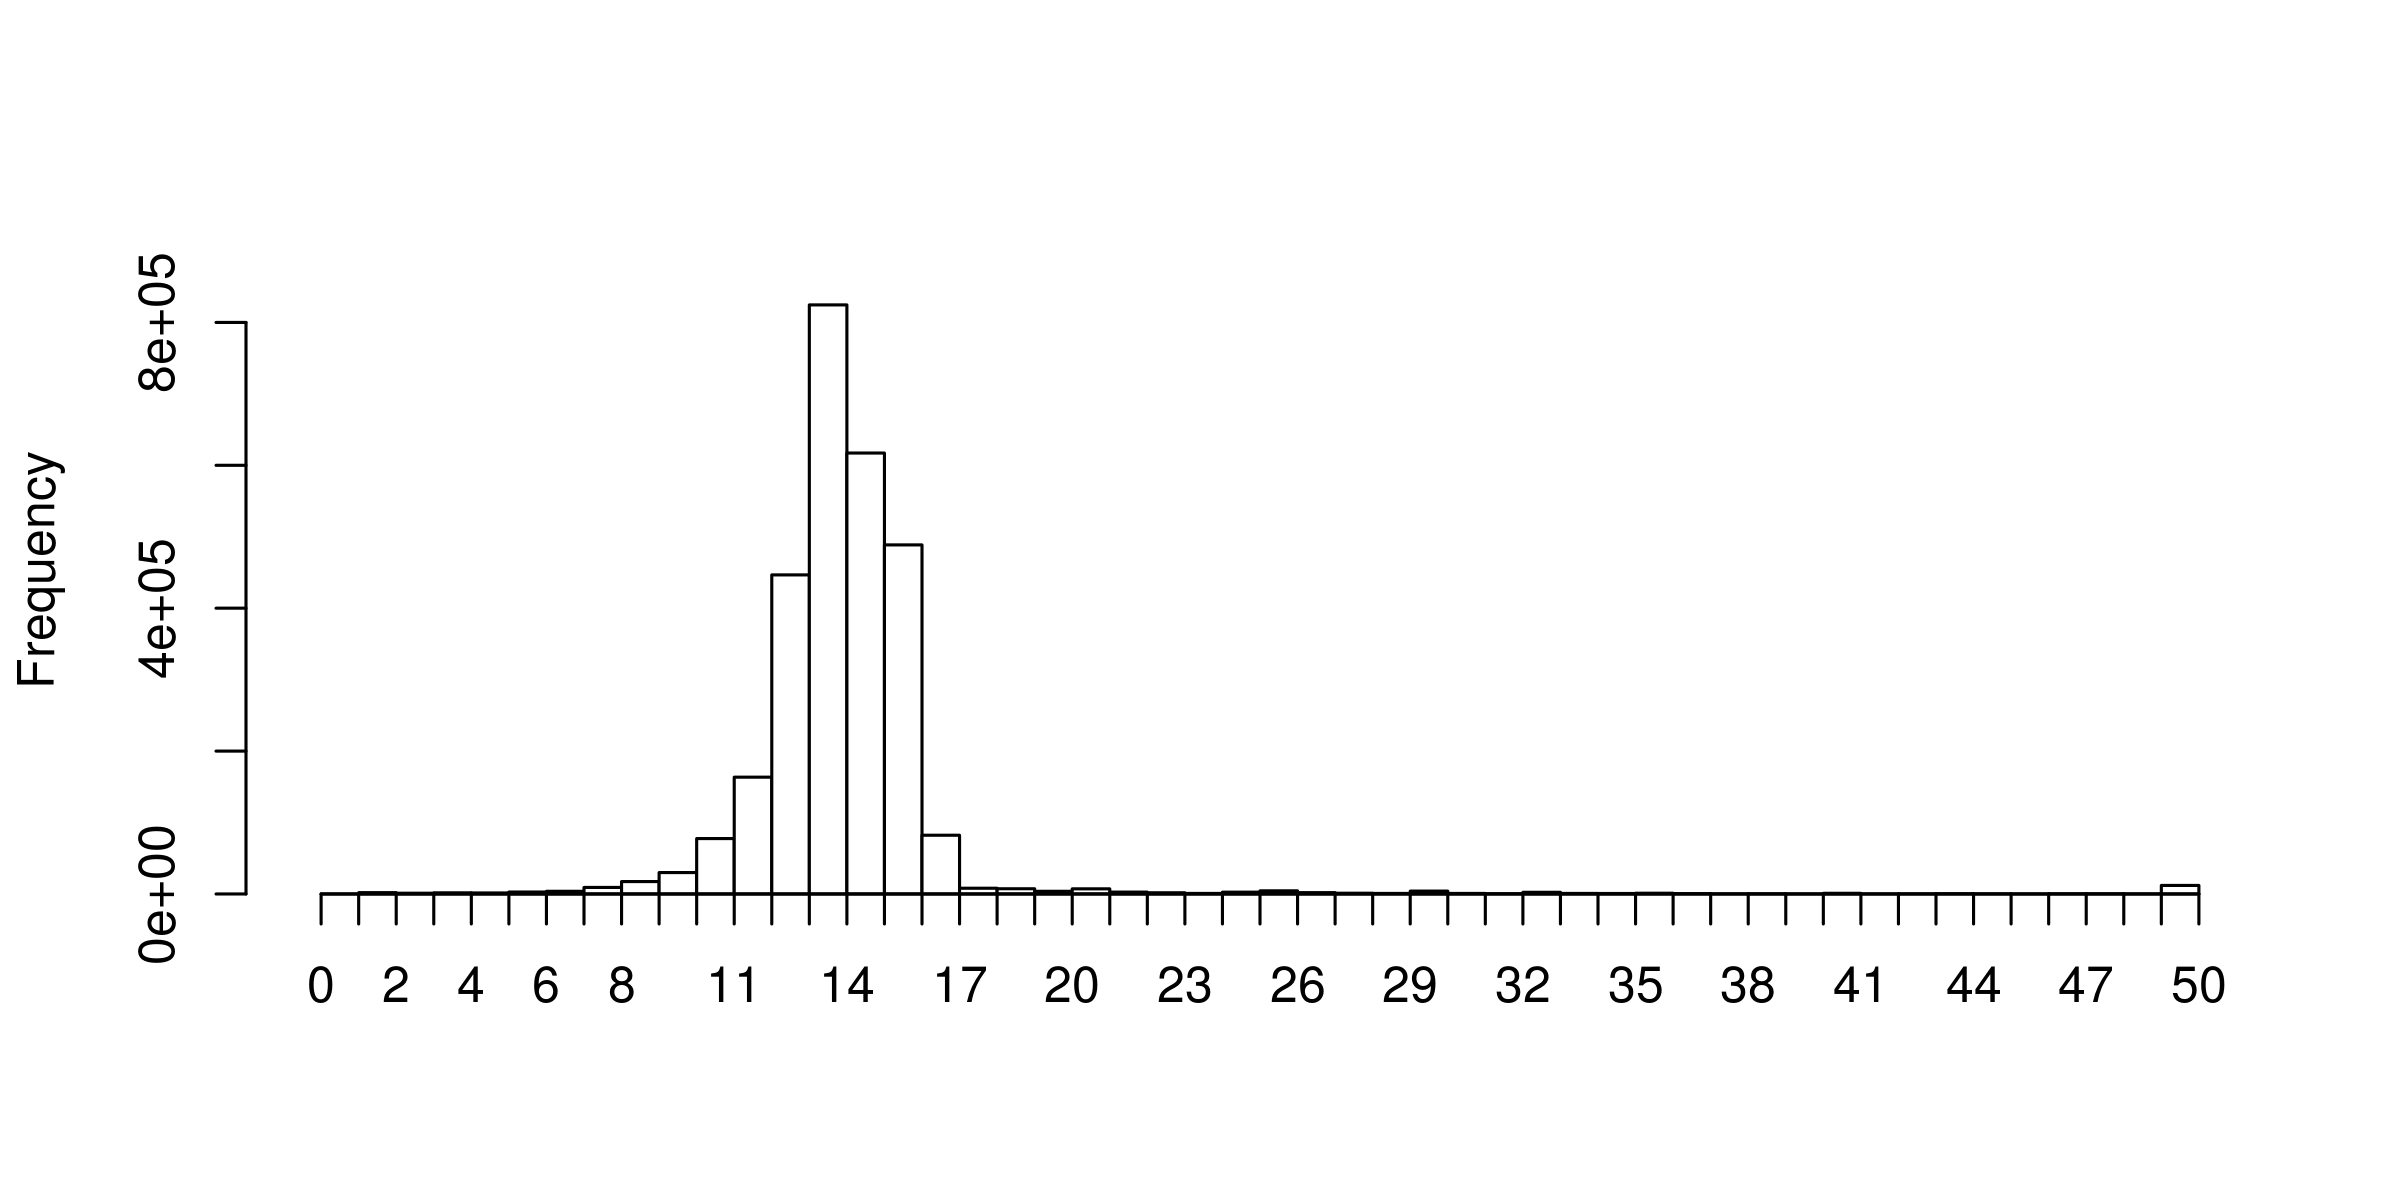
\includegraphics[width=0.8\textwidth]{de_novo/velvet_Rplot001.png}
\label{fig:SRS004748_coverage_hist}
\end{figure}

After choosing the expected coverage and the coverage cut-off, you can exit R by
typing:
\begin{lstlisting}
q()
\end{lstlisting}
\end{steps}

\begin{steps}
The weighted histogram suggests to me that the expected coverage is around 14
and that everything below 6 is likely to be noise. Some coverage is also
represented at around 20, 30 and greater 50, which might be contamination or
repeats (depending on the dataset), but at the moment this should not worry you.
To see the improvements, rerun velvetg first with \texttt{-cov\_cutoff} 6 and
after checking the N50 use only / add \texttt{-exp\_cov} 14 to the command line
option. Also keep a copy of the contigs file for comparison:
\begin{lstlisting}
cd ~/NGS/velvet/part1/SRS004748
time velvetg run_25 -cov_cutoff 6

# Make a copy of the run
cp run_25/contigs.fa run_25/contigs.fa.1

time velvetg run_25 -exp_cov 14
cp run_25/contigs.fa run_25/contigs.fa.2

time velvetg run_25 -cov_cutoff 6 -exp_cov 14
cp run_25/contigs.fa run_25/contigs.fa.3
\end{lstlisting}
\end{steps}

\begin{questions}
What is the N50 with no parameter:

What is the N50 with \texttt{-cov\_cutoff} 6:

What is the N50 with \texttt{-exp\_cov} 14:

What is the N50 with \texttt{-cov\_cutoff} 6 \texttt{-exp\_cov} 14:

Did you notice a variation in the time velvetg took to run? If so, can you
explain why that might be?

\end{questions}

\begin{steps}
You were running \texttt{velvetg} with the \texttt{-exp\_cov} and
\texttt{-cov\_cutoff} parameters. Now try to experiment using different
cut-offs, expected parameters and also explore other settings (e.g.
\texttt{-max\_coverage}, \texttt{-max\_branch\_length}, \texttt{-unused\_reads},
\texttt{-amos\_file}, \texttt{-read\_trkg} or see \texttt{velvetg} help menu).
\end{steps}

\begin{questions}
Make some notes about the parameters you've played with and the results you
obtained. Please also comment on the \texttt{-max\_coverage} and
\texttt{-max\_branch\_length} parameters.

\vspace{4\questionspacing}

\end{questions}


\begin{note}
In particular, look at the \texttt{-amos\_file} parameter which instructs
\texttt{velvetg} to create a version of the assembly that can be processed and
viewed with a program called AMOS Hawkeye. Another program, called tablet, can
also understand and display the AMOS file. For now, we will take a look at
Hawkeye.
\end{note}

\begin{steps}
Run velvetg with just \texttt{-cov\_cutoff} 6 but requesting an amos file:
\begin{lstlisting}
velvetg run_25 -cov_cutoff 6 -amos_file yes
\end{lstlisting}

Now convert the AMOS message file \texttt{velvet\_asm.afg} into an AMOS bank and
view the assembly using AMOS Hawkeye.
\begin{lstlisting}
bank-transact -c -b run_25/velvet_asm.bnk -m run_25/velvet_asm.afg
hawkeye run_25/velvet_asm.bnk
\end{lstlisting}

Once the file has loaded in Hawkeye, select and display one of the longer
contigs. Select the Contigs tab on the top of Hawkeye and take a closer look at
the Contigs information. Note the lack of Read information and the one
dimensional nature of the Contigs display. Close down Hawkeye when you have seen
enough and delete the AMOS bank file.
\begin{lstlisting}
rm -r run_25/velvet_asm.bnk
\end{lstlisting}

\end{steps}

\begin{steps}
Now rerun velvetg adding the additional parameter \texttt{-exp\_cov} 14 with no
need to save any files as the AMOS file needs to be changed.
\begin{lstlisting}
velvetg run_25 -cov_cutoff 6 -exp_cov 14 -amos_file yes
\end{lstlisting}

Again, convert the AMOS message file into an AMOS bank and view the assembly
using Hawkeye or tablet:
\begin{lstlisting}
bank-transact -c -b run_25/velvet_asm.bnk -m run_25/velvet_asm.afg
hawkeye run_25/velvet_asm.bnk
\end{lstlisting}

\begin{figure}[H]
\centering
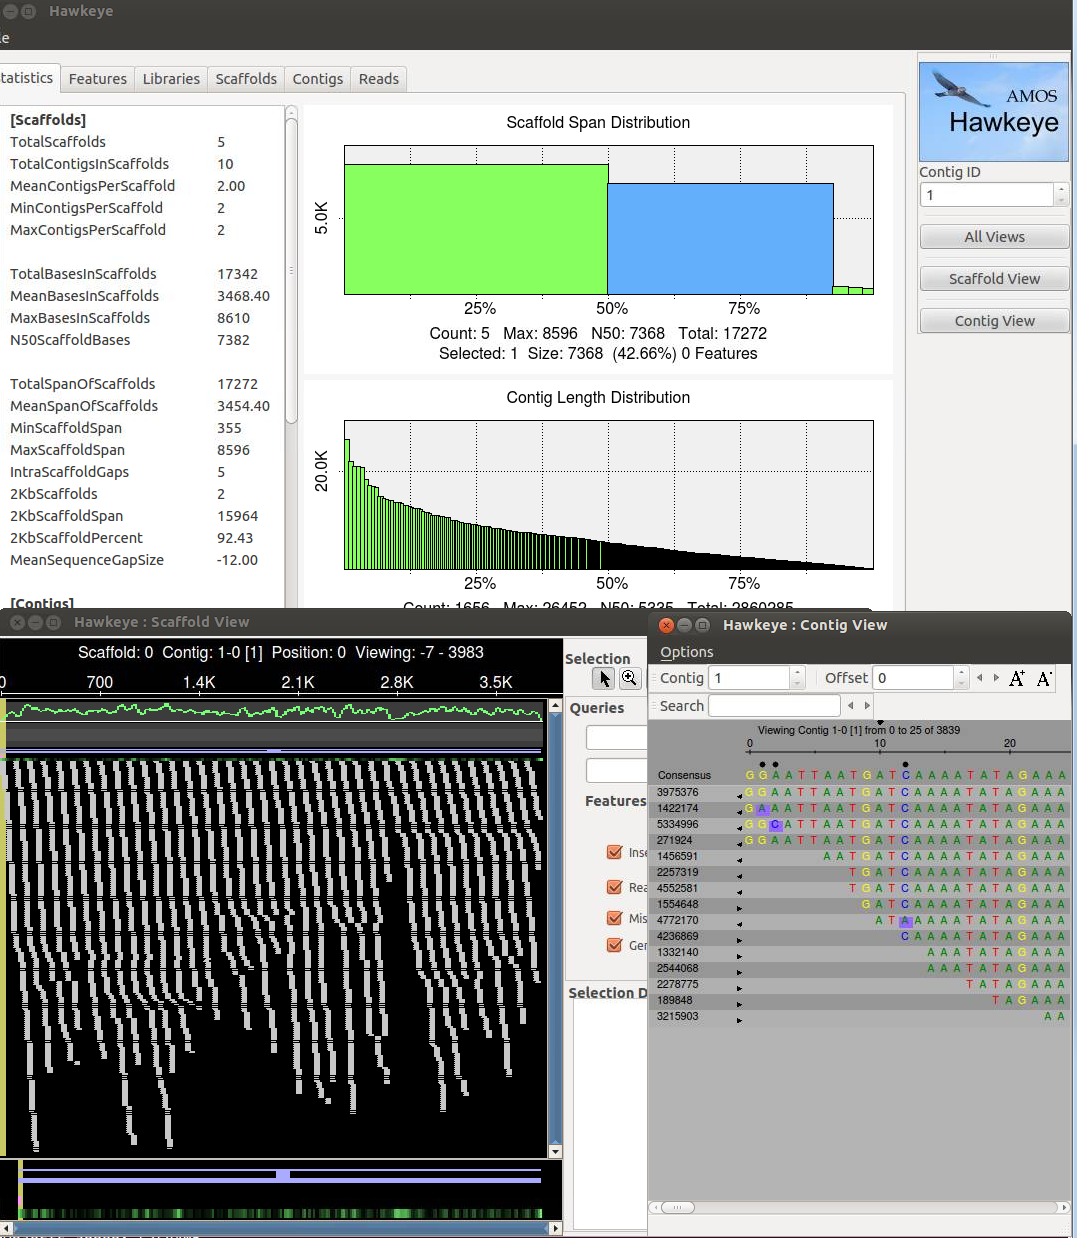
\includegraphics[width=0.8\textwidth]{de_novo/hawkeye_single_ended.png}
\caption{You should get a similar looking result with Hawkeye. If you are happy that you explored enough functionality, close down Hawkeye and continue with the exercise.}
\label{fig:hawkeye_single_ended}
\end{figure}

\end{steps}

\begin{questions}
Why do you think there was read information only for the second use of Hawkeye
and tablet?
  
You may have noticed velvetg took a little longer with \texttt{-exp\_cov} 14 on.
Does this make sense?

\end{questions}


\begin{bonus}
If you want to explore the behaviour of velvet even further, you could
experiment with the following.

Reduce the sequence coverage by only choosing one input file for the assembly
e.g. \texttt{SRR022825.fastq.gz}

Increase the sequence coverage by downloading further files from the same ENA
sample SRS004748 \url{http://www.ebi.ac.uk/ena/data/view/SRS004748}.

\begin{questions}
How did the N50 change by a) reducing the coverage and b) increasing the coverage:

\vspace{4\questionspacing}

\end{questions}

\end{bonus}

\subsection{Simple Assembly Simulation}

\begin{notes}
The data for this section is from Staphylococcus aureus MRSA252, a genome
closely related to the genome that provided the short read data in the earlier
sections of this exercise. The sequence data this time is the fully assembled
genome. The genome size is therefore known exactly and is 2,902,619 bp.
\end{notes}

\begin{information}
In this exercise you will process the single whole genome sequence with velveth
and velvetg, look at the output only and go no further. The main intent of
processing this whole genome is to compute its N50 value. This must clearly be
very close to the ideal N50 value for the short reads assembly and so aid
evaluation of that assembly.
\end{information}

\begin{steps}
To begin, move back to the main directory for this exercise, make a
sub-directory for the processing of this data and move into it. All in one go,
this would be:
\begin{lstlisting}
cd ~/NGS/velvet/part1/ 
mkdir MRSA252 
cd MRSA252
\end{lstlisting}

Next, you need to download the genome sequence from
\url{http://www.ensemblgenomes.org/} which holds five new sites, for bacteria,
protists, fungi, plants and invertebrate metazoa. You could browse for the data
you require or use the file which we have downloaded for you. For the easier of
these options, make and check a soft link to the local file and with the
commands:
\begin{lstlisting}
ln -s ~/NGS/Data/s_aureus_mrsa252.EB1_s_aureus_mrsa252.dna.chromosome.Chromosome.fa.gz ./
ls -l
\end{lstlisting}

\end{steps}

\begin{notes}
Usually Velvet expects relatively short sequence entries and for this reason has
a read limit of 32,767 bp per sequence entry. As the genome size is 2,902,619 bp
- longer as the allowed limit and does not fit with the standard settings into
velvet. But like the maximum k-mer size option, you can tell Velvet during
compile time, using \texttt{LONGSEQUENCES=Y}, to expect longer input sequences
than usual. I already prepared the executable which you can use by typing
\texttt{velveth\_long} and \texttt{velvetg\_long}.
\end{notes}

\begin{steps}
Now, run \texttt{velveth\_long}, using the file you either just downloaded or created a
soft link to as the input:
\begin{lstlisting}
velveth_long run_25 25 -fasta.gz -long s_aureus_mrsa252.EB1_s_aureus_mrsa252.dna.chromosome.Chromosome.fa.gz
velvetg_long run_25
\end{lstlisting}

\end{steps}

\begin{questions}
What is the N50?

How does the N50 compare to the previous single end run (SRS004748)?
  
Does the total length differ from the input sequence length?
  
What happens when you rerun velvet with a different k-mer length?

\end{questions}



\section{Assembling Paired-end Reads}

\begin{note}
The data you will examine in this exercise is again from Staphylococcus aureus
which has a genome of around 3MB. The reads are Illumina paired end with an
insert size of 350 bp.

The required data can be downloaded from the SRA. Specifically, the run data
(SRR022852) from the SRA Sample SRS004748.

\center{\url{http://www.ebi.ac.uk/ena/data/view/SRS004748}}

\end{note}

\begin{information}
The following exercise focuses on preparing the paired-end FASTQ files ready for
velvet, using velvet in paired-end mode and comparing results with velvet's
'auto' option.
\end{information}

\begin{steps}
First move to the directory you made for this exercise and make a suitable named
directory for the exercise:
\begin{lstlisting}
cd ~/NGS/velvet/part2 
mkdir SRS004748 
cd SRS004748
\end{lstlisting}

There is no need to download1 the read files, as they are already stored
locally. You will simply create a soft link to this pre-downloaded data using
the following commands:
\begin{lstlisting}
ln -s ~/NGS/Data/SRR022852_?.fastq.gz ./
\end{lstlisting}

It would be interesting to monitor the way that the programs you will run
utilize your computer's resources, particularly memory. A simple way to do this
is to open a second terminal and in it type:
\begin{lstlisting}
top
\end{lstlisting}
\end{steps}

\begin{note}
\texttt{top} is a program that continually monitors all the processes running on
your computer, showing the resources used by each. Alternatively you could use a
system monitor from your operating system as well. Leave this running and refer
to it at intervals, especially when programs appear to be taking a long time, of
just whenever your curiosity gets the better of you. You should find that as
this practical progresses, memory usage will increase significantly, but
hopefully not beyond the capacity of your workstation.

Now, back to the first terminal, you are ready to run \texttt{velveth} and \texttt{velvetg}. The
reads are \texttt{-shortPaired} this time and for the first run you should not use any
parameters for \texttt{velvetg}.
\end{note}

\begin{information}
From this point on, where it will be informative, time
your runs. This is very easy to do, just prefix the command to run the program
with the command \texttt{time}. This will cause UNIX to report how long the program took
to complete its task.
\end{information}

\begin{steps}
Set the two stages of velvet running, whilst you watch the memory usage as
reported by \texttt{top}. time the \texttt{velvetg} stage. The commands to enter
are:
\begin{lstlisting}
velveth run_25 25 -fmtAuto -create_binary -shortPaired -separate SRR022852_1.fastq.gz SRR022852_2.fastq.gz
time velvetg run_25
\end{lstlisting}

\end{steps}

\begin{questions}
Have you found what \texttt{-fmtAuto} and \texttt{-create\_binary} do? (see help menu)

Comment on the use of memory and CPU for \texttt{velveth} and \texttt{velvetg}?
 
How long did \texttt{velvetg} take?

\end{questions}

\begin{steps}
Next, after saving your \texttt{contigs.fa} file from being overwritten, set the
cut-off parameters that you investigated in the previous exercise and rerun
\texttt{velvetg}.
time and monitor the use of resources as previously. Start with
\texttt{-cov\_cutoff 16} thus:
\begin{lstlisting}
mv run_25/contigs.fa run_25/contigs.fa.0
time velvetg run_25 -cov_cutoff 16
\end{lstlisting}

Up until now, \texttt{velvetg} has ignored the paired-end information. Now try
running
\texttt{velvetg} with both \texttt{-cov\_cutoff 16} and \texttt{-exp\_cov 26}, but first save your \texttt{contigs.fa}
file. By using \texttt{-cov\_cutoff} and \texttt{-exp\_cov}, \texttt{velvetg}
tries to estimate the insert length, which you will see in the \texttt{velvetg}
output. The command is, of course:
\begin{lstlisting}
mv run_25/contigs.fa run_25/contigs.fa.1
time velvetg run_25 -cov_cutoff 16 -exp_cov 26
\end{lstlisting}

\end{steps}

\begin{questions}
Comment on the time required, use of memory and CPU for \texttt{velvetg}?
  
Which insert length does Velvet estimate?

\end{questions}

\begin{steps}
Next try running \texttt{velvetg} in `paired-end mode`. This entails running \texttt{velvetg}
specifying the insert length with the parameter \texttt{-ins\_length} set to 350. Even
though velvet estimates the insert length it is always advisable to check /
provide the insert length manually as velvet can get the statistics wrong due
to noise. Just in case, save your last version of \texttt{contigs.fa}. The commands are:
\begin{lstlisting}
mv run_25/contigs.fa run_25/contigs.fa.2
time velvetg run_25 -cov_cutoff 16 -exp_cov 26 -ins_length 350
mv run_25/contigs.fa run_25/contigs.fa.3
\end{lstlisting}
\end{steps}

\begin{questions}
How fast was this run?

\end{questions}

\begin{steps}
Take a look into the Log file.
\end{steps}

\begin{questions}
What is the N50 value for the \texttt{velvetg} runs using the switches:\\
\texttt{-cov\_cutoff 16}

\texttt{-cov\_cutoff 16 -exp\_cov 26}

\texttt{-cov\_cutoff 16 -exp\_cov 26 -ins\_length 350}

\end{questions}

\begin{steps}
Try giving the \texttt{-cov\_cutoff} and/or \texttt{-exp\_cov} parameters the
value \texttt{auto} - the \texttt{velvetg} help output could show you how. The
information Velvet prints during running includes information about the values
used (coverage cut-off or insert length) when using the \texttt{auto} option.
\end{steps}

\begin{questions}
Which coverage values does Velvet choose (hint: look at the output which velvet
produces while running)?

How does the N50 value change?
\end{questions}

\begin{steps}
Run \texttt{gnx} on all the \texttt{contig.fa} files you have generated in the
course of this exercise. The command will be:
\begin{lstlisting}
gnx -min 100 -nx 25,50,75 run_25/contigs.fa*
\end{lstlisting}
\end{steps}

\begin{questions}
For which runs are there Ns in the \texttt{contigs.fa} file and why? 
  
Comment on the number of contigs and total length generated for each run.
\end{questions}


\begin{bonus}
Similar to the single-end assembly you created previously, we can output a
paired-end assembly as an AMOS message format file. This file can then be
converted into an AMOS bank and viewed using AMOS Hawkeye.
\begin{lstlisting}
time velvetg run_25 -cov_cutoff 16 -exp_cov 26 -ins_length 350 -amos_file yes -read_trkg yes 
time bank-transact -c -b run_25/velvet_asm.bnk -m run_25/velvet_asm.afg         
hawkeye run_25/velvet_asm.bnk
\end{lstlisting}

\begin{questions}
Looking at the scaffold view of a contig, comment on the proportion of happy
mates to compressed mates.

What is the mean and standard deviation of the insert size report in the
Libraries tab of Hawkeye?

Look at the actual distribution of insert sizes for this library. Can you
explain where there is a difference between the mean and SD reported in those
two places?
\end{questions}

\begin{steps}
You can get AMOS to re-estimate the mean and SD of insert sizes. First, close
Hawkeye and then run the following commands before reopening the AMOS bank to
see what has changed.
\begin{lstlisting}
asmQC -b run_25/velvet_asm.bnk -scaff -recompute -update -numsd 2
hawkeye run_25/velvet_asm.bnk
\end{lstlisting}
\end{steps}

\begin{questions}
Looking at the scaffold view of a contig, comment on the proportion of happy
mates to compressed mates.

What is the mean and standard deviation of the insert size report in the
Libraries tab of Hawkeye?

Look at the actual distribution of insert sizes for this library. Does the mean
and SD reported in each of those two places now match?
\end{questions}
\end{bonus}

\subsection{Data Quality}
\begin{note}
As discussed previously, fastq format files include quality assessment of each
called base. As also mentioned earlier, velvet does not use this information
directly. However, by taking into account the quality of the read data, it
should be possible to both improve the efficiency (in terms of memory usage and
runtime) and the quality of the output.
\end{note}

\begin{information}
To investigate the effect of data quality, we will use the run data (SRR023408)
from the SRA experiment SRX008042. The reads are Illumina paired end with an
insert size of 92 bp.
\end{information}

\begin{steps}
As ever, move up a directory to the main directory for the whole of this
exercise and create and enter a new directory dedicated to this phase of the
exercise. The commands are:
\begin{lstlisting}
cd ~/NGS/velvet/part2 
mkdir SRX008042 
cd SRX008042
\end{lstlisting}

Create soft links to the read data files we downloaded for you from the SRA with
the command:
\begin{lstlisting}
ln -s ~/NGS/Data/SRR023408_?.fastq.gz ./
\end{lstlisting}
\end{steps}

\begin{note}
To look at the quality scores, you could use a tool called FastQC to process and
present the scores in a compact manner of basic statistics. FastQC can be
downloaded from:

\center{\url{http://www.bioinformatics.bbsrc.ac.uk/projects/fastqc/}}

Where there are links to an excellent manual and an even more excellent youtube
video. I hope to show you the video and recommend you keep the manual pages open
whilst you are using FastQC in this exercise.
\end{note}

\begin{steps}
Start up FastQC Graphical User Interface (GUI) to examine your compressed fastq
files by typing:
\begin{lstlisting}
fastqc &
\end{lstlisting}
\end{steps}

\begin{note}
The & sets FastQC running as a background job, thus freeing your terminal for
further commands if required. FastQC emerges as a big blank window.
\end{note}

\begin{steps}
Open both your compressed fastq files as was done in the video (Choose Open from
the File pull down menu, browse to your files, select them both and click OK).
Look at tabs for both files:
\end{steps}

\begin{figure}[H]
\centering
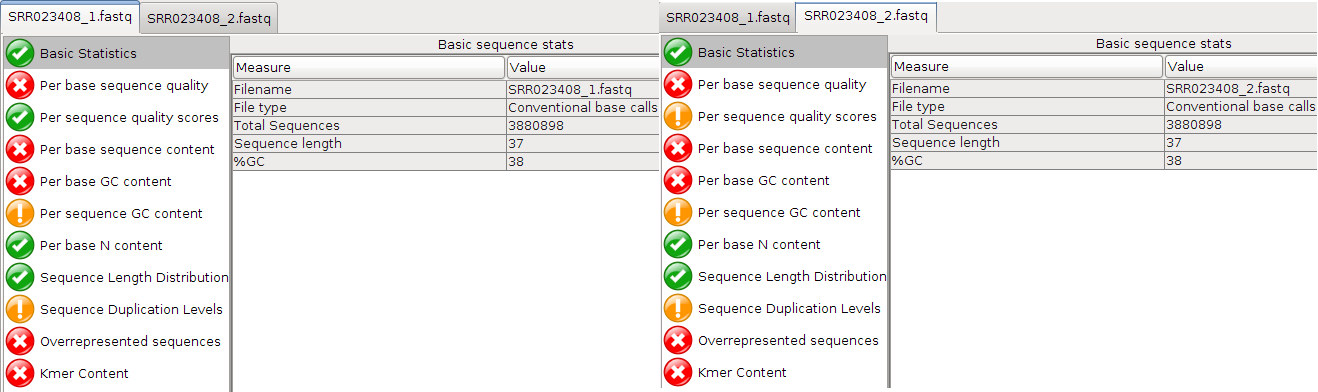
\includegraphics[width=0.8\textwidth]{de_novo/paired_fastqc.png}
\label{fig:paired_fastqc}
\end{figure}

\begin{questions}
Are the quality scores the same for both files?

Which value varies?

Take a look at the Per base sequence quality for both files. Did you note that it is not good for either file?

At which positions would you cut the reads off?

Why does the quality deteriorate towards the end of the read?

Does it make sense to trim the start?
\end{questions}

\begin{steps}
Have a look at the other options that fastqc offers. Make good use of the Help
to remind you of what you learned from the video. I suggest you open the Help
window and keep it on your screen, open at the relevant page, as you browse
through the fastqc possibilities.
\end{steps}

\begin{questions}
Which other statistics could you use to support your trimming strategy?
\end{questions}

\begin{figure}[H]
\centering
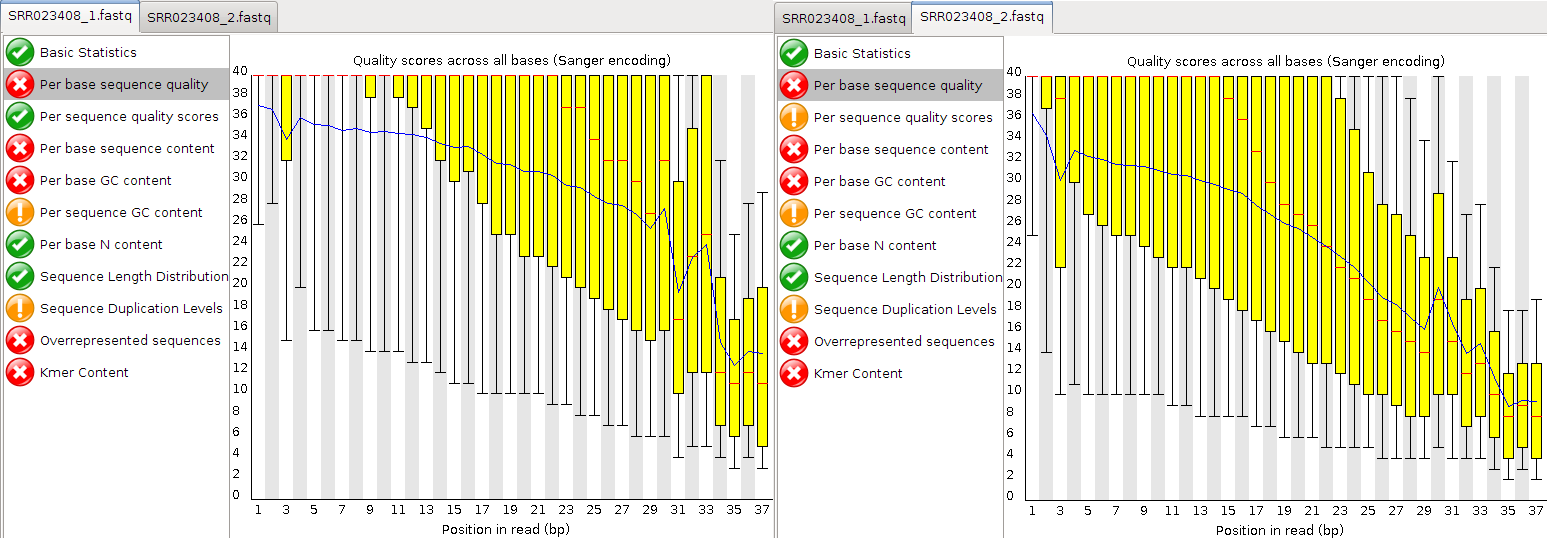
\includegraphics[width=0.8\textwidth]{de_novo/paired_fastqc_quality_plots.png}
\label{fig:paired_fastqc_quality_plots}
\end{figure}

\begin{steps}
Once you have decided how it might be sensible to trim your reads, close down
fastqc by selecting Exit from the File pull down menu. Now apply the knife to
your reads with \texttt{fastx\_trimmer} from the FASTX-Toolkit. However, you will
first need to decompress the FASTQ files. The usage of the tool can be found
here:

\url{http://hannonlab.cshl.edu/fastx_toolkit/commandline.html#fastx_trimmer_usage}

The suggestion (hopefully not far from your own thoughts?) is that you trim your
reads as follows:

\begin{lstlisting}
gunzip < SRR023408_1.fastq.gz > SRR023408_1.fastq
gunzip < SRR023408_2.fastq.gz > SRR023408_2.fastq
fastx_trimmer -Q 33 -f 4 -l 32 -i SRR023408_1.fastq -o SRR023408_trim1.fastq 
fastx_trimmer -Q 33 -f 3 -l 29 -i SRR023408_2.fastq -o SRR023408_trim2.fastq
\end{lstlisting}

Now run velveth with a k-mer value of 21 for both the untrimmed and trimmed read
files in \texttt{-shortPaired} mode. Separate the output of the two executions
of \texttt{velveth} into suitably named directories, followed by
\texttt{velvetg}. The commands would be:
\begin{lstlisting}
velveth run_21 21 -fmtAuto -create_binary -shortPaired -separate SRR023408_1.fastq SRR023408_2.fastq
time velvetg run_21

velveth run_21trim 21 -fmtAuto -create_binary -shortPaired -separate SRR023408_trim1.fastq SRR023408_trim2.fastq
time velvetg run_21trim
\end{lstlisting}
\end{steps}

\begin{questions}
What are the times for the two \texttt{velvetg} runs?

What N50 scores did you achieve?

What were the overall effects of trimming?
\end{questions}

\begin{steps}
The evidence is that trimming improved the assembly. The thing to do surely, is
to run velvetg with the \texttt{-cov\_cutoff} and \texttt{-exp\_cov}. In order
to use \texttt{-cov\_cutoff} and \texttt{-exp\_cov} sensibly, you need to
investigate with R, as you did in the previous exercise, what parameter values
to use. To start up R and produce the weighted histograms, type:
\begin{lstlisting}
R --no-save
library(plotrix) 
data <- read.table("run_21/stats.txt", header=TRUE) 
data2 <- read.table("run_21trim/stats.txt", header=TRUE) 
x11()
par(mfrow=c(1,2))
weighted.hist(data$short1_cov, data$lgth, breaks=0:50)
weighted.hist(data2$short1_cov, data2$lgth, breaks=0:50)
\end{lstlisting}

\begin{figure}[H]
\centering
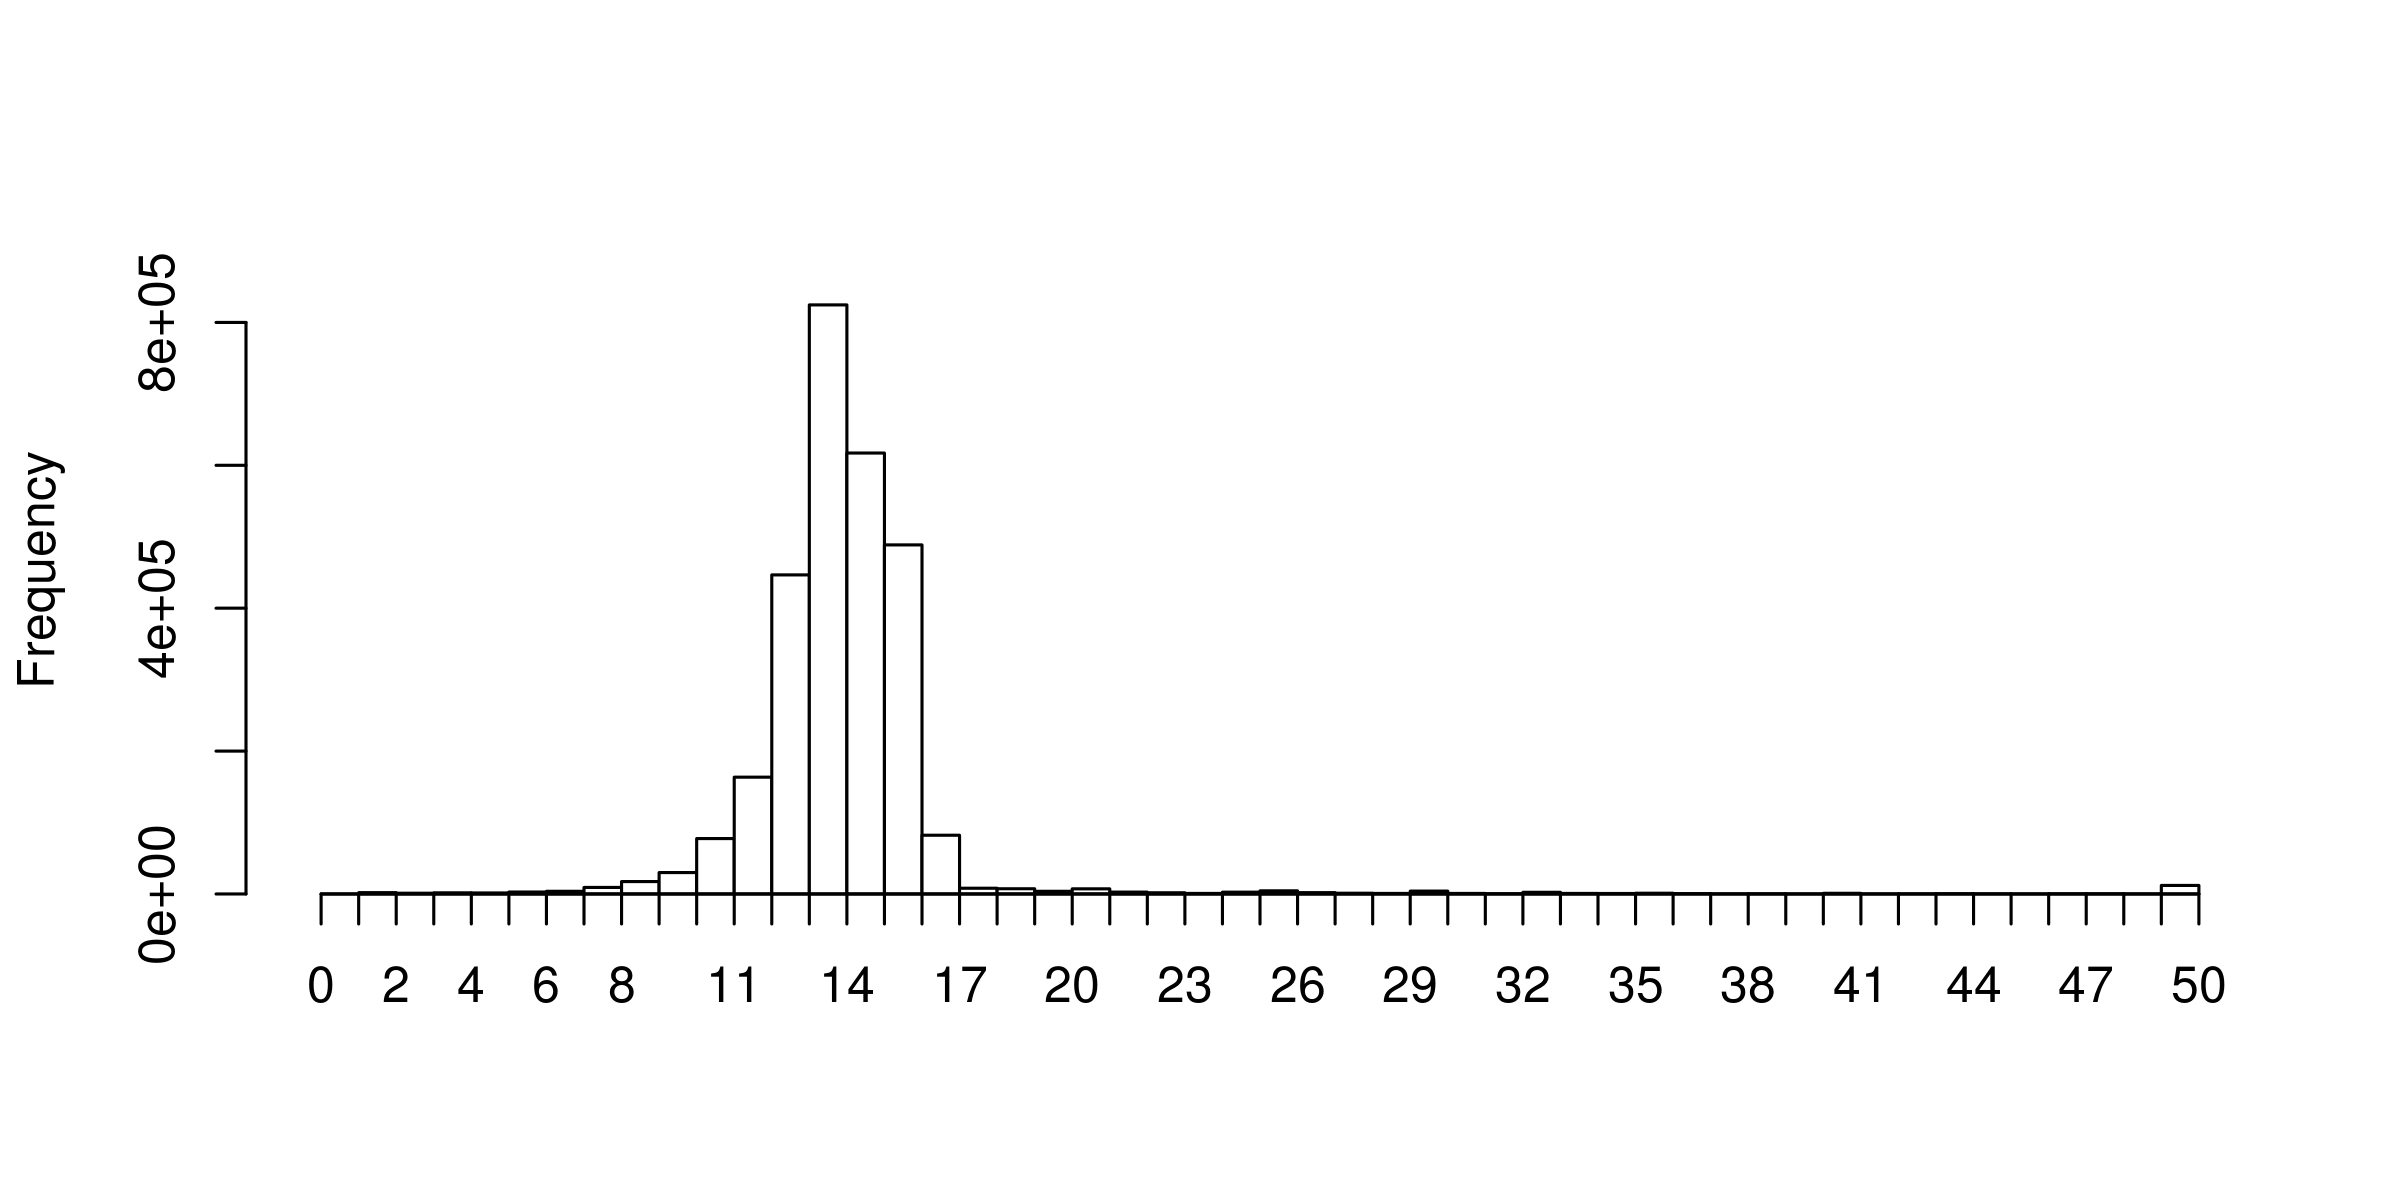
\includegraphics[width=0.8\textwidth]{de_novo/velvet_Rplot001.png}
\label{fig:velvet_Rplot001}
\end{figure}

One histogram suggests to me an expected coverage of around 13 with a coverage
cut-off of around 7. The trimmed histogram instead suggests an expected coverage
of around 9 with a coverage cut-off of around 5. If you disagree, feel free to
try different settings, but first leave R before running velvetg:
\begin{lstlisting}
q()

time velvetg run_21 -cov_cutoff 7 -exp_cov 13 -ins_length 92
time velvetg run_21trim -cov_cutoff 5 -exp_cov 9 -ins_length 92
\end{lstlisting}

\end{steps}

\begin{questions}
How good does it look now? Comment on:\\ 
Runtime

Memory

k-mer choice (Can you use kmer 31 for a read of length 30 bp?)

Does less data mean 'worse' results?
  
How would a smaller/larger Kmer size behave?
\end{questions}

\begin{steps}
Compare the results, produced during the last exercises, with each other:

\begin{table}[H]
  \centering
  %\caption{FastQC Basic Statistics table}
    \begin{tabular*}{0.9\textwidth}{l|l|l|l}
    \toprule
    Metric & SRR022852 & SRR023408 & SRR023408.trimmed \\
    \midrule
    Overall Quality (1-5) & & & \\[0.5\questionspacing]
    \hline
    bp Coverage & & & \\[0.5\questionspacing]
    \hline
    k-mer Coverage & & & \\[0.5\questionspacing]
    \hline
    N50 (k-mer used) & & & \\[0.5\questionspacing]
    \bottomrule
    \end{tabular}%
  \label{tab:comparison}%
\end{table}%

\end{steps}

\begin{questions}
What would you consider as the 'best' assembly?

If you found a candidate, why do you consider it as 'best' assembly?
\end{questions}


\section{Assembling Long (454) Read}

\begin{note}
The data you will examine in this exercise is again from Staphylococcus aureus
which has a genome of around 3MB. The reads are 454 single end.

The required data can be downloaded from the SRA. Specifically, the run data
(SRR000892,SRR000893) from the SRA Experiment SRX000181.

\center{\url{http://www.ebi.ac.uk/ena/data/view/SRX000181}}
\end{note}

\begin{information}
The following exercise focuses on processing 454 long reads with velvet and how
this differs compared to short reads.
\end{information}

\begin{steps}
First move to the directory you made for this exercise and make a suitable named
directory for the exercise before downloading the read files:
\begin{lstlisting}
cd ~/NGS/velvet/part3
mkdir SRX000181
cd SRX000181
\end{lstlisting}

The downloaded files can be used directly in velvet. To let velvet know that
these fastq files are long reads, you pass in the parameter \texttt{-long} by
using the commands:
\begin{lstlisting}
ln -s ~/NGS/Data/SRR000892.fastq.gz
ln -s ~/NGS/Data/SRR000893.fastq.gz
velveth run_25 25 -create_binary -fastq.gz -long *.fastq.gz
time velvetg run_25
\end{lstlisting}
\end{steps}

\begin{questions}
Take a look at the stats.txt file. Which columns are used compared to short reads and why?

Which N50 do you get?

How long did the velvetg run take?
\end{questions}

\begin{steps}
The right thing to do is to run velvetg setting the cut-offs. But for long reads
there is an option called \texttt{-long\_cov\_cutoff} to filter them
independently because of the difference in usage in velvet. To investigate with
R, as you did in the previous exercises, start up R and produce the weighted
histogram using the column \texttt{long\_cov} by typing:
\begin{lstlisting}
R --no-save
library(plotrix) 
data <- read.table("run_25/stats.txt", header=TRUE) 
x11() 
weighted.hist(data$long_cov, data$lgth, breaks=0:50)
\end{lstlisting}

\begin{figure}[H]
\centering
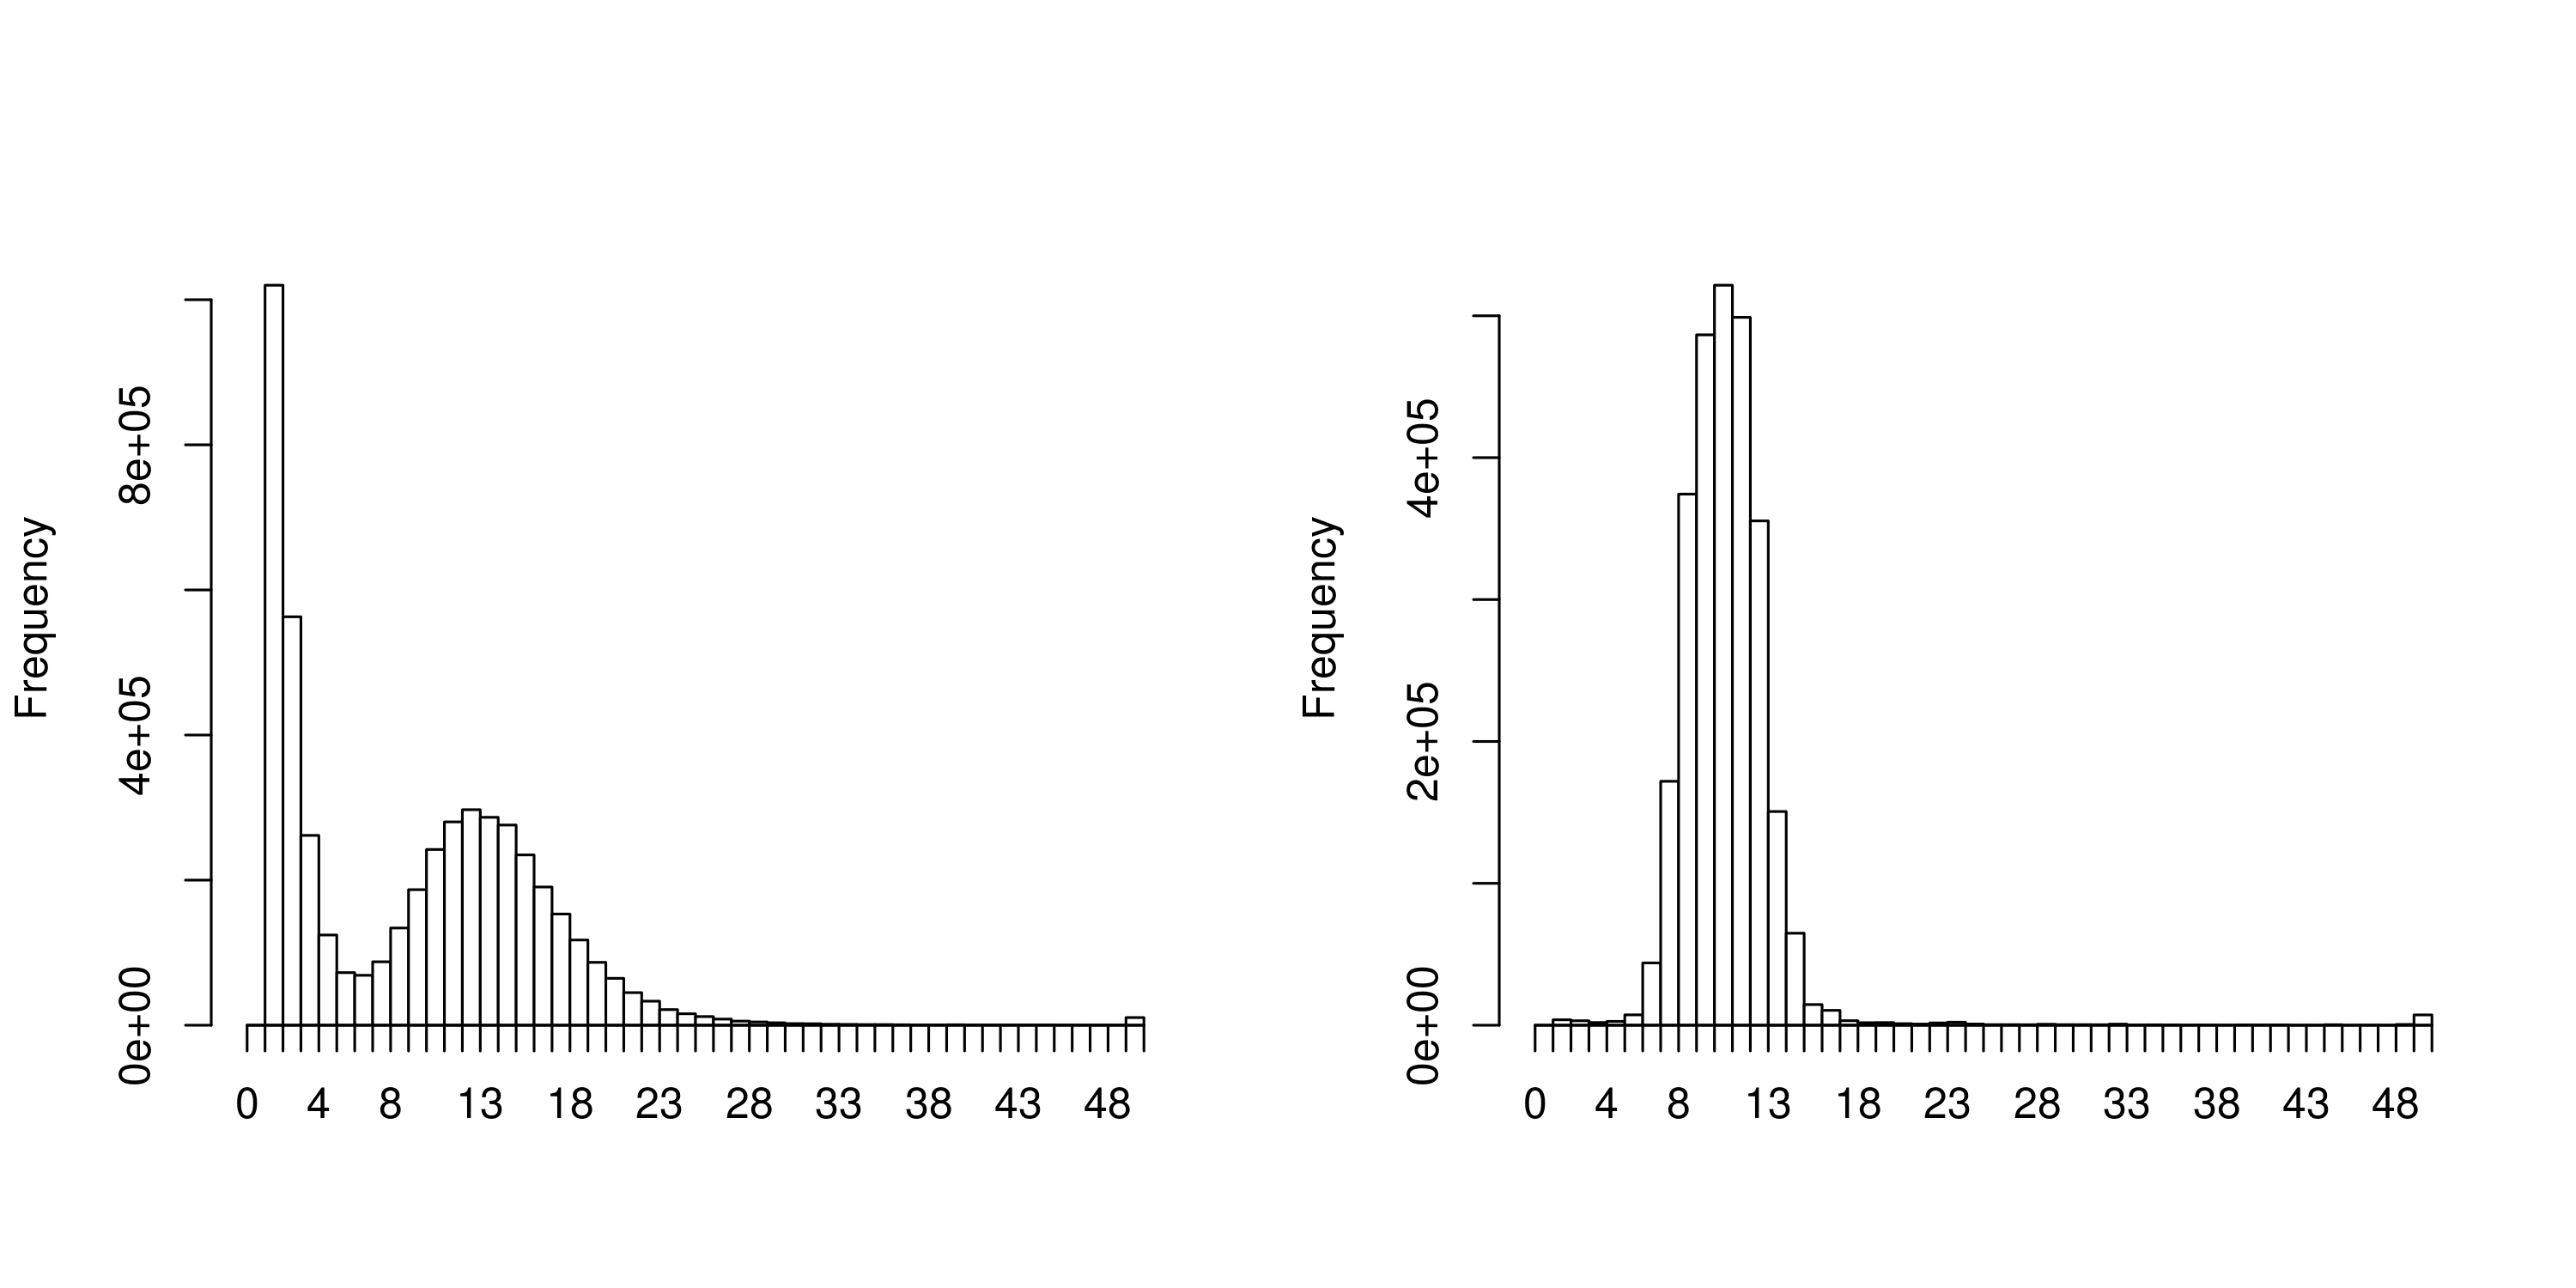
\includegraphics[width=0.8\textwidth]{de_novo/velvet_Rplot002.png}
\label{fig:velvet_Rplot002}
\end{figure}

For me the histogram suggests to me to choose a coverage cut-off of around 9
with an expected coverage of about 19. If you disagree, feel free to try
different settings, but first leave R before running \texttt{velvetg} with the
coverage parameters typing:
\begin{lstlisting}
q()

cp run_25/contigs.fa run_25/contigs.fa.0

time velvetg run_25 -long_cov_cutoff 9
cp run_25/contigs.fa run_25/contigs.fa.1

time velvetg run_25 -long_cov_cutoff 9 -exp_cov 19
cp run_25/contigs.fa run_25/contigs.fa.2

gnx -min 100 -nx 25,50,75 run_25/contigs.fa.*
\end{lstlisting}

\end{steps}

\begin{questions}
What is the N50 and runtime using:
\texttt{-long\_cov\_cutoff 9}
  
\texttt{-long\_cov\_cutoff 9 -exp\_cov 19}
  
other runs?
    
Which other parameters could improve the assembly quality for long reads?

What do you think about assembling 454 reads with Velvet?
\end{questions}


\section{Assembling Mixed Insert Length Libraries}

\begin{note}
Like the previous examples, the data you will examine in this exercise is again
from Staphylococcus aureus which still has a genome of around 3MB. The reads are
Illumina paired end with an insert size of 170 bp and 350 bp.

You already downloaded the required reads from the SRA in previous exercises.
Specifically, the run data (SRR022863, SRR022852) from the SRA Study SRP001086.

\center{\url{http://www.ebi.ac.uk/ena/data/view/SRP001086}}
\end{note}

\begin{information}
The following exercise focuses on handing two insert length libraries with
velvet and the changes you have to look out for.
\end{information}

\begin{steps}
First move to the directory you made for this exercise, make a suitable named
directory for the exercise and check if all the files are in place:
\begin{lstlisting}
cd ~/NGS/velvet/part3
mkdir SRP001086
cd SRP001086
ln -s ~/NGS/Data/SRR022863_?.fastq.gz ./
ln -s ~/NGS/Data/SRR022852_?.fastq.gz ./
\end{lstlisting}

Now run \texttt{velveth} and \texttt{velvetg} using the appropriate command line
options by typing:
\begin{lstlisting}
time velveth run_25 25 -fmtAuto -create_binary -shortPaired -separate SRR022863_1.fastq.gz SRR022863_1.fastq.gz -shortPaired2 -separate SRR022852_1.fastq.gz SRR022852_2.fastq.gz
time velvetg run_25
\end{lstlisting}

The right thing to do is to run velvetg setting the cut-offs. To investigate
with R, as you did in the previous exercises, start up R and produce the
weighted histogram using the columns \texttt{short1\_cov} and
\texttt{short2\_cov} by typing:
\begin{lstlisting}
R --no-save
library(plotrix) 
data <- read.table("run_25/stats.txt", header=TRUE) 
weighted.hist(data$short1_cov+data$short2_cov, data$lgth, breaks=0:70)
\end{lstlisting}

\begin{figure}[H]
\centering
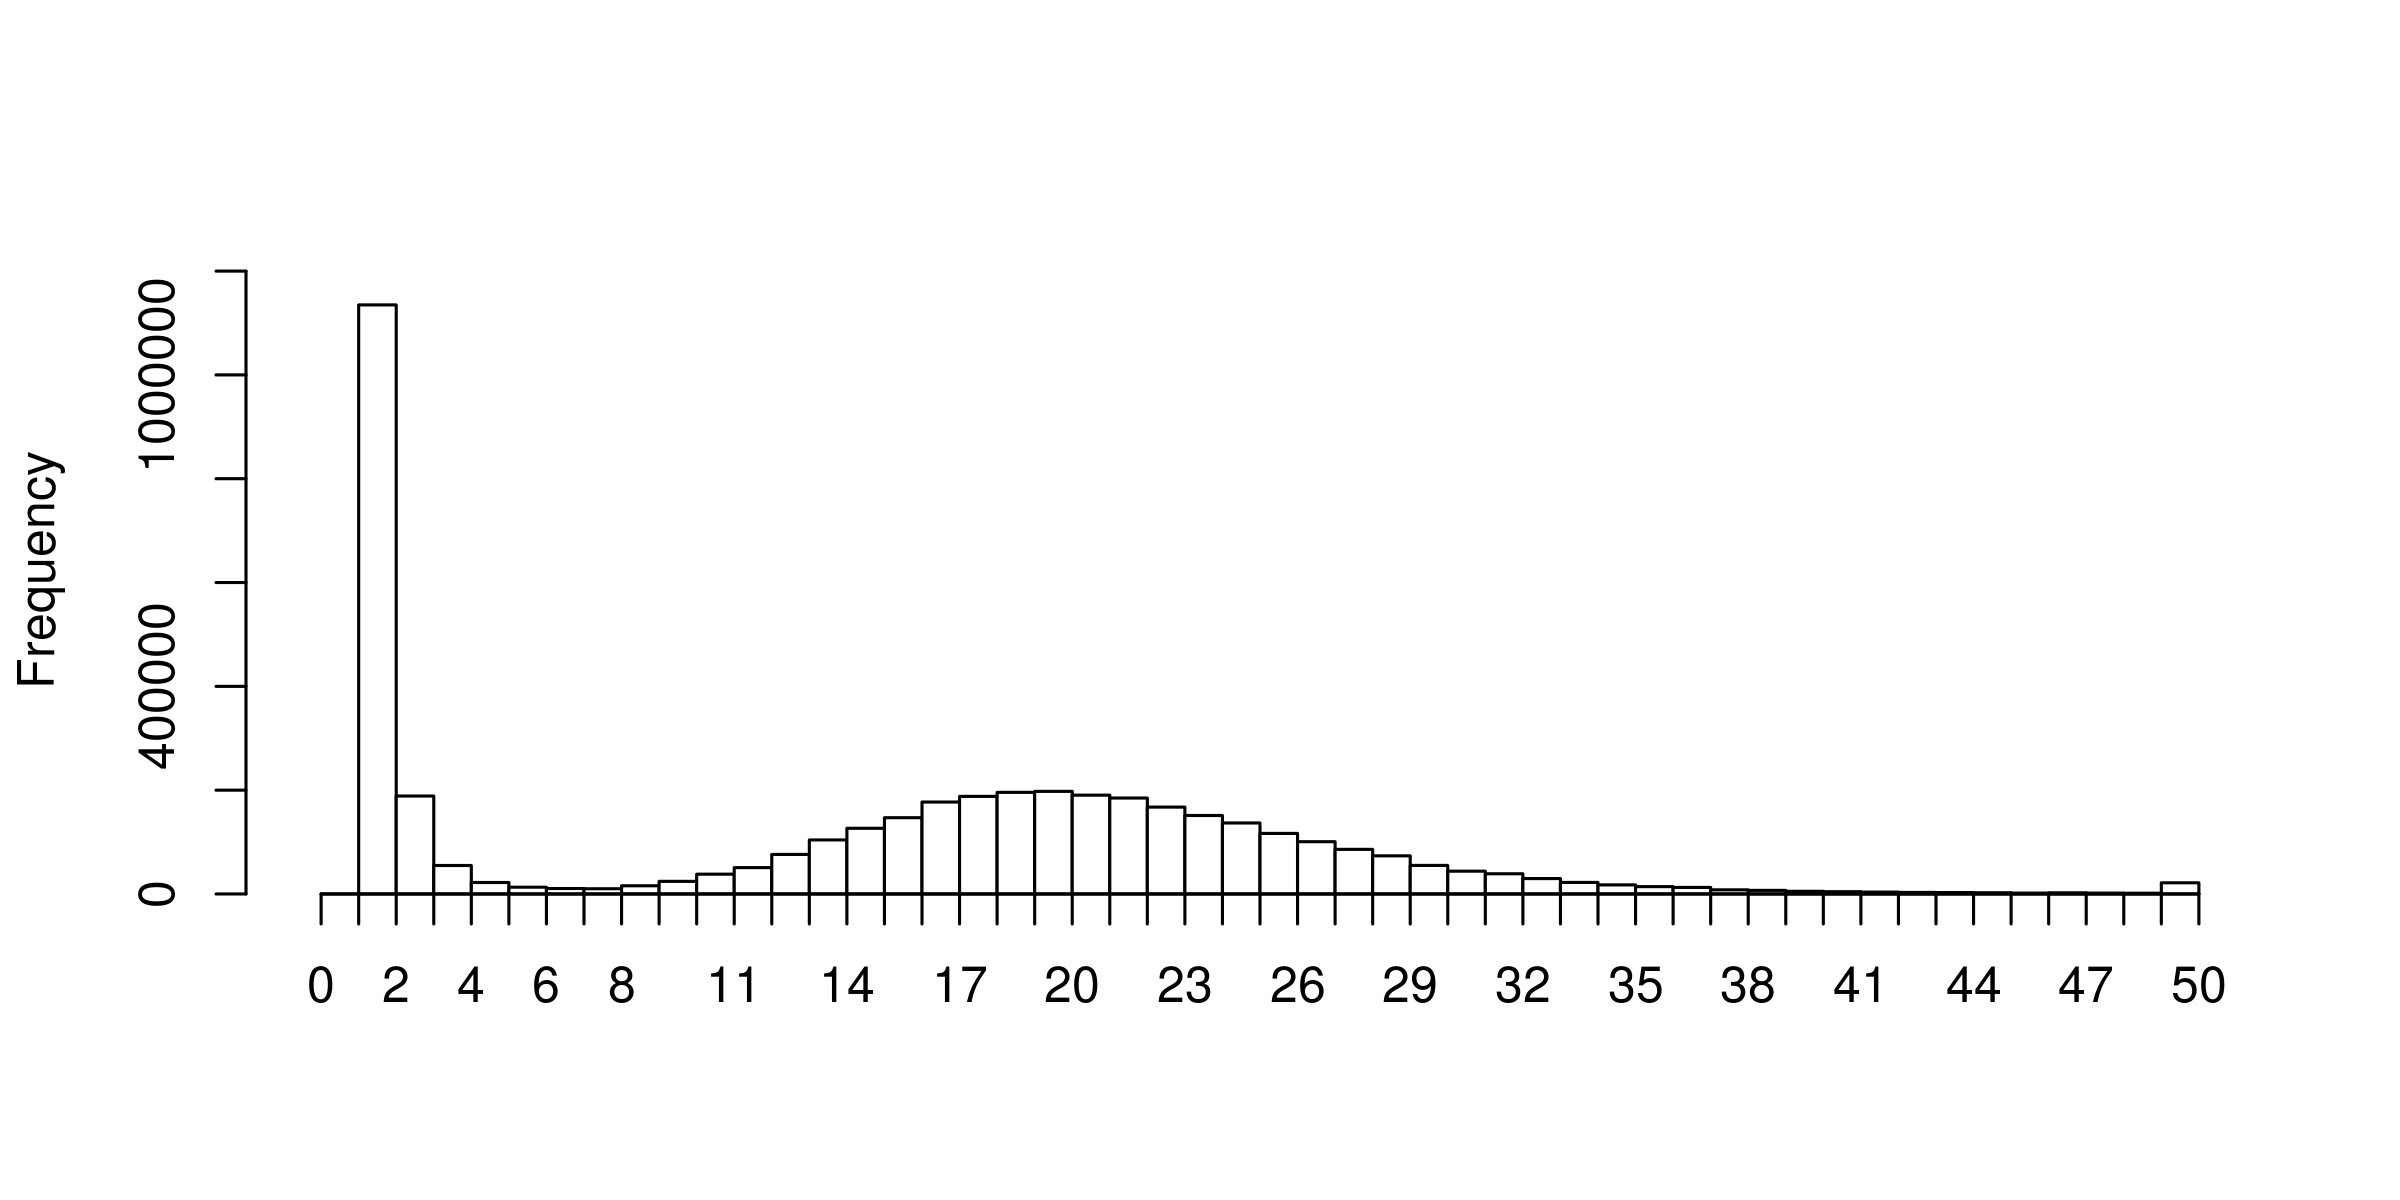
\includegraphics[width=0.8\textwidth]{de_novo/velvet_Rplot003.png}
\label{fig:velvet_Rplot003}
\end{figure}

For me the histogram suggests to me to choose a coverage cut-off of around 20
with an expected coverage of about 36. If you disagree, feel free to try
different settings, but first leave R before running velvetg with the coverage
parameters typing:
\begin{lstlisting}
q()

cp run_25/contigs.fa run_25/contigs.fa.0

time velvetg run_25 -cov_cutoff 20 
cp run_25/contigs.fa run_25/contigs.fa.1

time velvetg run_25 -cov_cutoff 20 -exp_cov 36 
cp run_25/contigs.fa run_25/contigs.fa.2

time velvetg run_25 -cov_cutoff 20 -exp_cov 36 -ins_length 170 -ins_length2 350
cp run_25/contigs.fa run_25/contigs.fa.3

gnx -min 100 -nx 25,50,75 run_25/contigs.fa.*
\end{lstlisting}

\end{steps}

\begin{questions}
What N50 did you get?

How did the runtime/results compare to one paired-end library runs?

How many different libraries would you be able to run with this velvet version?

Would you be able to add a single-end library as well with this velvet version?
\end{questions}

\begin{bonus}
Find and download a different insert length library
% TODO: \footnote affects the width of the shaded box - \renewcommand{\footnote}?
\footnotemark[1]
from the
study SRP001086 and recompile velvet to allow the use of three insert length
libraries. Maybe you could use the library you trimmed during previous
exercises. You should be able to find these files here:
\texttt{~/NGS/velvet/part2/SRX008042/SRR023408\_trim?.fastq}. If you don't still
have these files, you can find a copy of them here:
\texttt{~/NGS/Data/SRR023408\_trim?.fastq}.
Use the fresh compiled Velvet version with the three (two provided and one
downloaded library) to assemble the genome.
\begin{questions}
Does the extra library make any difference?
 
How does the overall coverage change?
 
Any other comments?
\end{questions}
\footnotetext[1]{Paired insert
lengths can be found on the NCBI SRA page in the library section (Nominal
length) e.g. \url{http://www.ncbi.nlm.nih.gov/sra?term=SRR022866}}
\end{bonus}

\begin{advanced}
\section{Hybrid Assembly}
\begin{note}
Like the previous examples, the data you will examine in this exercise is again
from Staphylococcus aureus which has a genome of around 3MB. The reads are 454
single end and Illumina paired end with an insert size of 170 bp.
You already downloaded the required reads from the SRA in previous exercises.
Specifically, the run data (SRR022863, SRR000892, SRR000893) from the SRA
experiments SRX007709 and SRX000181.
\end{note}

\begin{information}
The following exercise focuses on handing 454 long reads and paired-end reads
with velvet and the differences in setting parameters.
\end{information}

\begin{steps}
First move to the directory you made for this exercise, make a suitable named
directory for the exercise and check if all the three files are in place:
\begin{lstlisting}
cd ~/NGS/velvet/part3
mkdir SRR000892-SRR022863 
cd SRR000892-SRR022863
ln -s ~/NGS/Data/SRR00089[2-3].fastq.gz ./   
ln -s ~/NGS/Data/SRR022863_?.fastq.gz ./
\end{lstlisting}
\end{steps}

\begin{warning}
The following command will run for a LONG time. This indicated the amount of
calculations being preformed by Velvet to reach a conclusion. To wait for velvet
to finish would exceed the time available in this workshop, but it is up to you
to either let it run over night or kill the process by using the key combination
\texttt{CTRL+c}.
\begin{lstlisting}
velveth run_25 25 -fmtAuto -create_binary -long SRR00089?.fastq.gz -shortPaired -separate SRR022863_1.fastq.gz SRR022863_2.fastq.gz
time velvetg run_25
\end{lstlisting}

\begin{steps}
If you have decided to continue, we already inspected the weighted histograms
for the short and long read library separately, you can reuse this for the
cut-off values:
\begin{lstlisting}
time velvetg run_25 -cov_cutoff 7 -long_cov_cutoff 9
\end{lstlisting}
\end{steps}

\begin{questions}
What are your conclusions using velvet in an hybrid assembly?
\end{questions}

\end{warning}




\end{advanced}











\chapterstyle{workshop}

%
% End of modules
% Switch back to normal workshop chapter styling
%
\chapterstyle{workshop}

\end{document}
